% !TEX encoding = UTF-8 Unicode

\documentclass[12pt,a4j,titlepage]{ltjsarticle}
\usepackage{semi}


% \title{}
% \author{}
% \date{}

\begin{document}

\begin{titlepage}
  \begin{center}
  
    \vspace*{20truept}
    
    {\LARGE 2024年度 卒業論文} 
    
    \vspace*{75truept}
    
    {\Huge  論文タイトル考える} %論文タイトル

    \vspace{10truept}

    {\Huge } %論文タイトル 長い場合 改行1

    \vspace{10truept}

    {\Huge } %論文タイトル 改行2

    \vspace{85truept}
    
    {\LARGE 指導教員 須田 宇宙 准教授}
    
    \vspace{60truept}
    
    {\LARGE 千葉工業大学 情報ネットワーク学科}
    
    \vspace{15truept}
    
    {\LARGE 須田研究室}
    
    \vspace{70truept}
    
    {\LARGE 2132160 氏名 渡邉 理紗子 } % 氏名は消さない 学生番号 氏名 名前

    \vspace{70truept}
    
  \end{center}
  \begin{flushright}

    {\LARGE 提出日 2025年1月17日}
  
  \end{flushright}
\end{titlepage}

\setcounter{tocdepth}{3}
% 目次の出力
\tableofcontents
% 表目次
\listoftables
% 図目次
\listoffigures
\clearpage


% 1章
\section{緒言}
2018年に内閣府が提唱したsociety5.0ではグローバルにも通用するデジタル人材を求めている\cite{naikaku}.
グローバル化に対応した人材は2012年に文部科学省で発表された「大学で育成する人物像と大学政策」でも求められており,大学での人材育成についてまとめられている.
育成すべき能力として課題探求能力をはじめ,専門的知識,汎用的能力,人格形成を挙げている\cite{monka1}.
しかし,文部科学省は学習意欲の低下と,それに伴う自主学習時間の減少による大学生の学力低下を問題視しており\cite{monka2},大学での人材育成がなされていないといえる.

大学で育成すべき専門的知識は,高校生までに触れてこなかった新しい概念が出てくるため,知識の積み重ねが求められる.
そのため,配布される授業資料には難しい単語や説明が並び,学習する際に抵抗が生まれてしまうと考えられる.
その結果,知識が積み重ねられず,授業内容を理解しきれない.

インターネットは90年代から普及をはじめ,利用率は2013年で80\%を超えるようになった.
世代別の調査では20代のネットの利用率は98\%になっている\cite{somu6}.
また,日本では2007年にApple社のiPhoneが登場してから,2011年にスマートフォン(スマホ)が主流になった\cite{somu1}.
2017年にはスマホの所有率は75\%になり,パソコンの所有率を上回っている.
令和6年の調査ではスマホの所有率は90\%を超えた\cite{somu6}.
学生は行動をする際にスマホを頼ることが多くなり,自主学習においても教科書やノートではなくスマホを使用する場面が増えていると考えられる.
しかし,インターネット上には情報が多く,知識が点在しているため自主学習を始めるにはハードルが高いという問題がある.
そこで本研究では,「学習習慣がない学生には授業内容に沿った導入コンテンツが必要である」という仮説を立て,自主学習への繋がりについての検証を目的とする.

\clearpage

% 2章
\section{学生の学習状況}

% 2章 1節
\subsection{文部科学省で行われたアンケート}
文部科学省では大学の教育改善や国の政策立案など大学・国の双方においては様々な用途に活用することを目的として毎年短期大学も含めた大学生を対象に全国学生調査を行っている\cite{monka}.
全国学生調査は大学の授業の状況や大学での経験とその有用さ,大学教育を通じて知識・能力の習得,平均的な1週間の生活時間という4つの内容に分けて全45問の調査を行っている.
図\ref{fig:tyousa}は令和4年度の平均的な1週間の生活習慣という内容のうち予習・復習・課題など授業に関する学習状況という項目の調査結果である.
1週間の学習時間が5時間以下の学生は70\%を超えており,ほとんどの学生が1日当たりに換算すると40分も学習を行っていないことがわかる.

%図1
\begin{figure}[!htb]
  \centering
  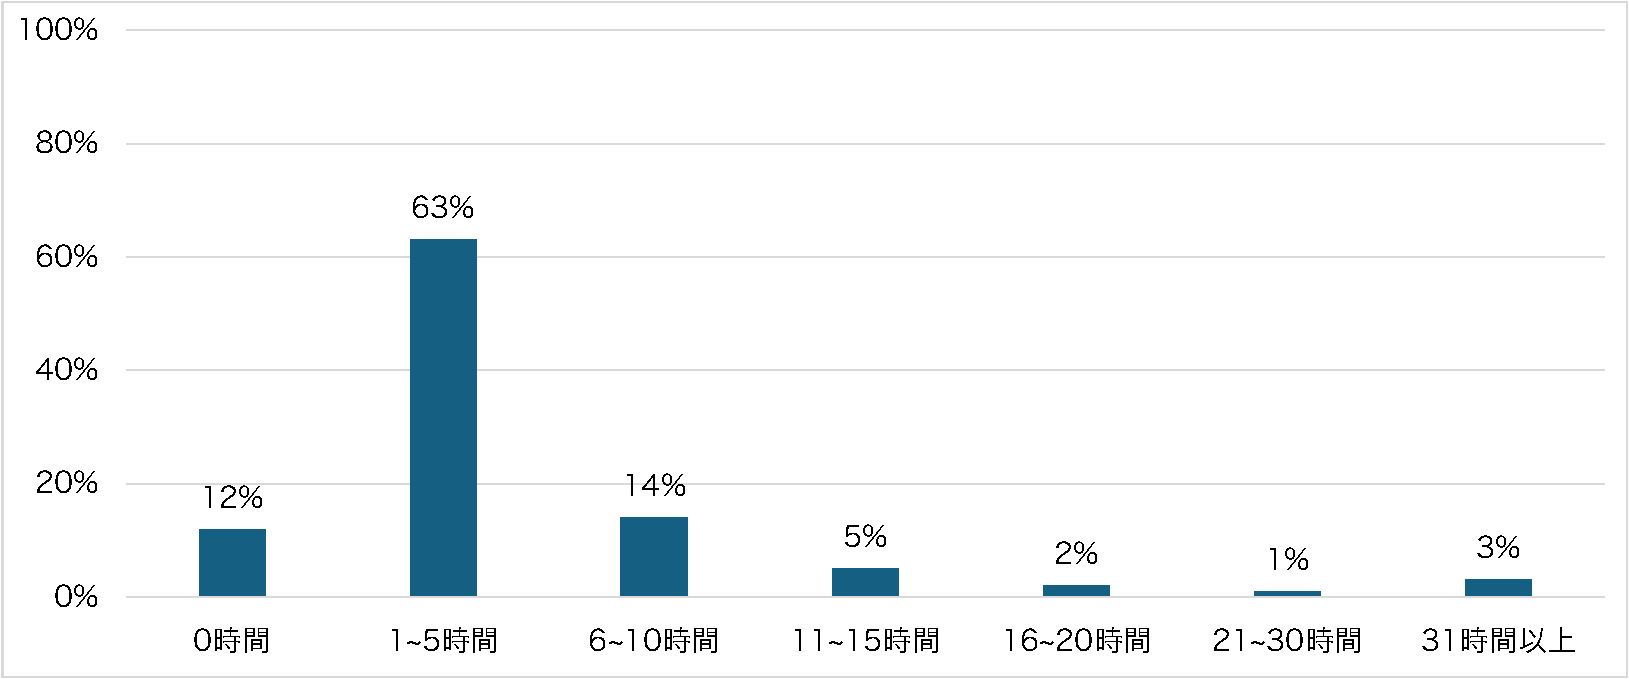
\includegraphics[width=15cm]{全国学生調査.pdf}
  \caption{1週間の予習・復習・課題など授業に関する学習時間}
  \label{fig:tyousa}
\end{figure}

%令和4年度の全国学生調査において,授業期間中の平均的な1週間の生活時間という項目では予習・復習・課題など授業に関する学習が5時間以下の学生が7割を超えていた.



% 2章 2節
\subsection{本校で行われたアンケート}
本校では学生の動向把握するとともに学生の意思を大学運営に反映させることを目的として年に1回学生生活アンケートが行われている.
学生生活アンケートには授業期間中の平均的な1週間の生活という項目に授業時間以外の学修時間や部活動/サークルなどの質問がある.
2023年の授業時間以外の学修時間という質問では学科や学年によって値にばらつきはあるが,全体の60\%ほどの学生が5時間以下の学習しか行えていないという結果が出ている\cite{chiba}.

\clearpage

% 3章 
\section{大学の授業について}
% 3章 1節
\subsection{大学設置基準における授業時間}
文部科学省には単位や授業時間など大学を設置するにあたって必要な最低限の基準をまとめた大学設置基準がある.
大学生の学習時間について大学設置基準で1単位当たり45時間の学習が必要であるとされている.
また,授業は10週又は15週にわたる期間を単位として行い,1単位当たり実験・実習では30-45時間,講義・演習では15-30時間を授業で扱うよう定められている.
10週間の期間の中で15時間を授業で扱った場合,1週間当たり3時間の自主学習を行い,残りの30時間を補う必要がある.

本校で開講されている科目は2時間で2単位であるため,90時間の学習を行う必要がある.
しかし,前期と後期に分かれており,各13週にわたって行われるため,授業では26時間ほどしか扱われていない.
そのため,残りの64時間を自主学習として行わなければならない.

% 3章 2節
\subsection{大学教育で育成すべき能力}
今日,日本では生産年齢人口の減少や技術革新等により,社会構造や雇用環境が急速に変化しており,今後どのように社会が変化していくかを予測することが困難になっている.
また,少子高齢化によって将来の日本を支える若者の人口が減少している.
そのことから,一人一人が持続可能な社会を支えることが求められており,その能力を生かして個人と社会の成長につながる新たな価値を生み出していくことが期待されている.
このことより文部科学省は,高度の専門知識を備えた人材やグローバル化に対応した人材の育成を目指しており,課題探求能力の他に学士力として専門的知識,汎用的能力,人材形成を大学で育成することを2012年から求めている.


%文部科学省では小学校から知識や技能の習得だけでなく,社会で必要な能力として思考力や判断力などの人間的能力の育成を掲げている.
%これらの育成のために学校での授業では主体的・対話的学習の深い学びを目指した取り組みが行われている.

\clearpage

% 4章 
\section{学習コンテンツ}

% 4章 1節
\subsection{ネット上の学習コンテンツ}
インターネットは90年代から普及し,近年では当たり前に存在するようになった.
図\ref{fig:net}は令和6年度に総務省で行われたインターネットの利用率であり,1997年から2023年にかけて大きく増加していることがわかる.
図\ref{fig:nendai}は年代階層別のインターネットの利用率であり,20代は98\%と30代,10代の次に高く,1日当たり約290分をインターネットの利用に割いている.
また,図\ref{fig:sumaho}はスマートフォンの保持率の推移であり,2023年の調査では90%がスマートフォンを所有していることがわかる\cite{somu6}.
これらのことから,日常的にスマートフォンを扱ってインターネットを利用していると考えられる.

インターネットが普及したことにより,動画配信やブログ,サイトなどの学習コンテンツが増加している.
動画配信の市場規模は2019年から2023年までの4年間で2925億円から5740億円まで拡大した\cite{somu2}.
%インターネットの普及によりブログやサイトは増加し,特にブログでは日本人の60\%が閲覧や書き込みをしていることが明らかになっている.
ブログでは,日本人の60\%が閲覧や書き込みをしていることが明らかになっている.
また,コロナの影響によりオンライン教育が発達し,コンピュータなどの情報技術を用いて学習するeラーニングは日本人の20\%が利用している\cite{somu2}.
動画配信やサイトなどのネット上の学習コンテンツは必要としている情報をすぐに得ることができるため,利用している学生が多いと考えられる.
しかし,情報の中には間違ったものや古いものがあるため,学生にとって正しい情報を選択することは難しい.

%図2
\begin{figure}[!htb]
  \centering
  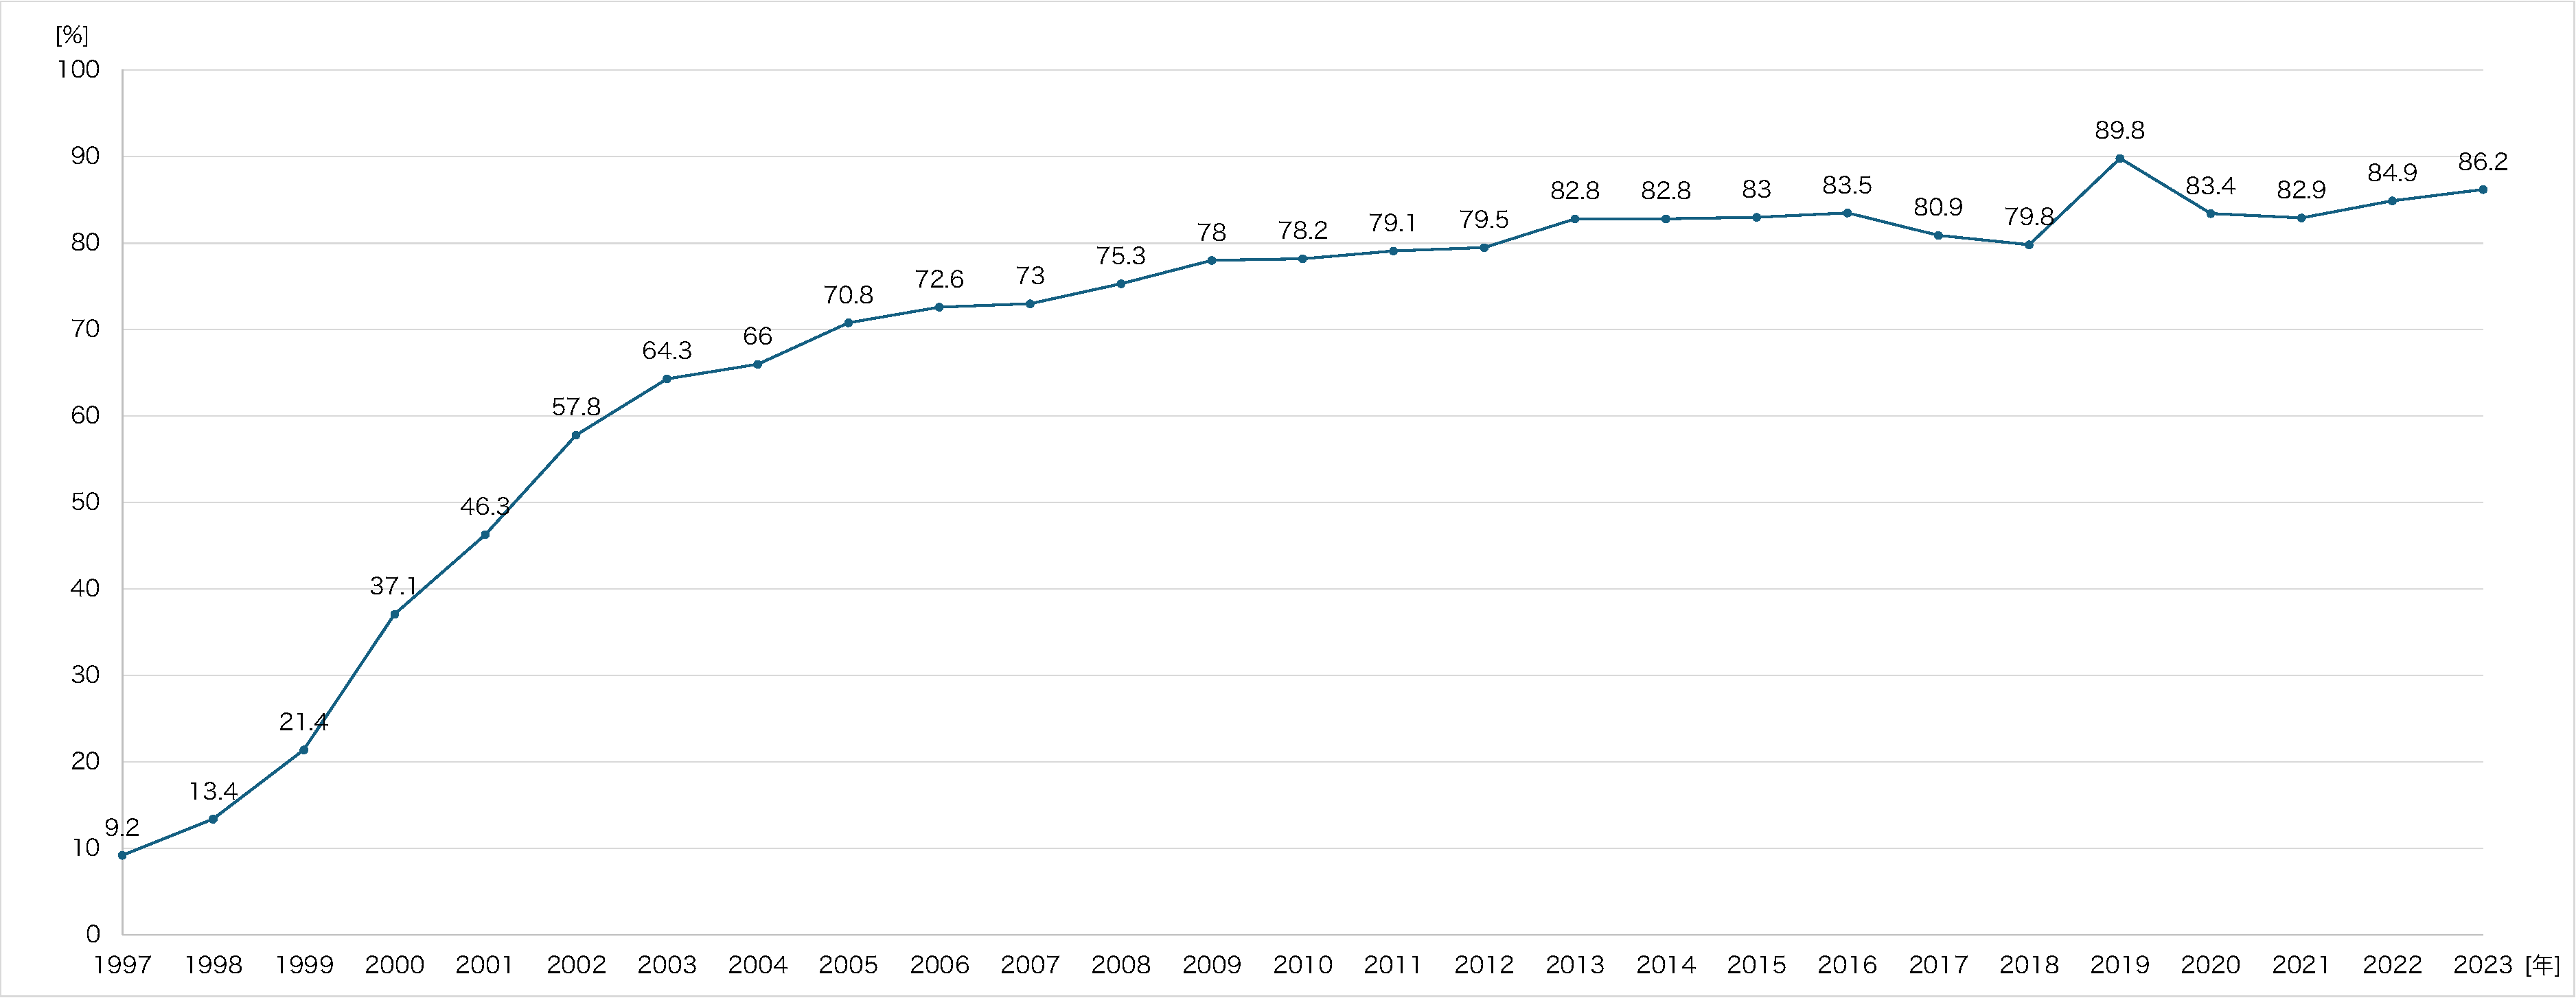
\includegraphics[width=15cm]{ネット利用率.pdf}
  \caption{インターネットの利用}
  \label{fig:net}
\end{figure}

%図3
\begin{figure}[!htb]
  \centering
  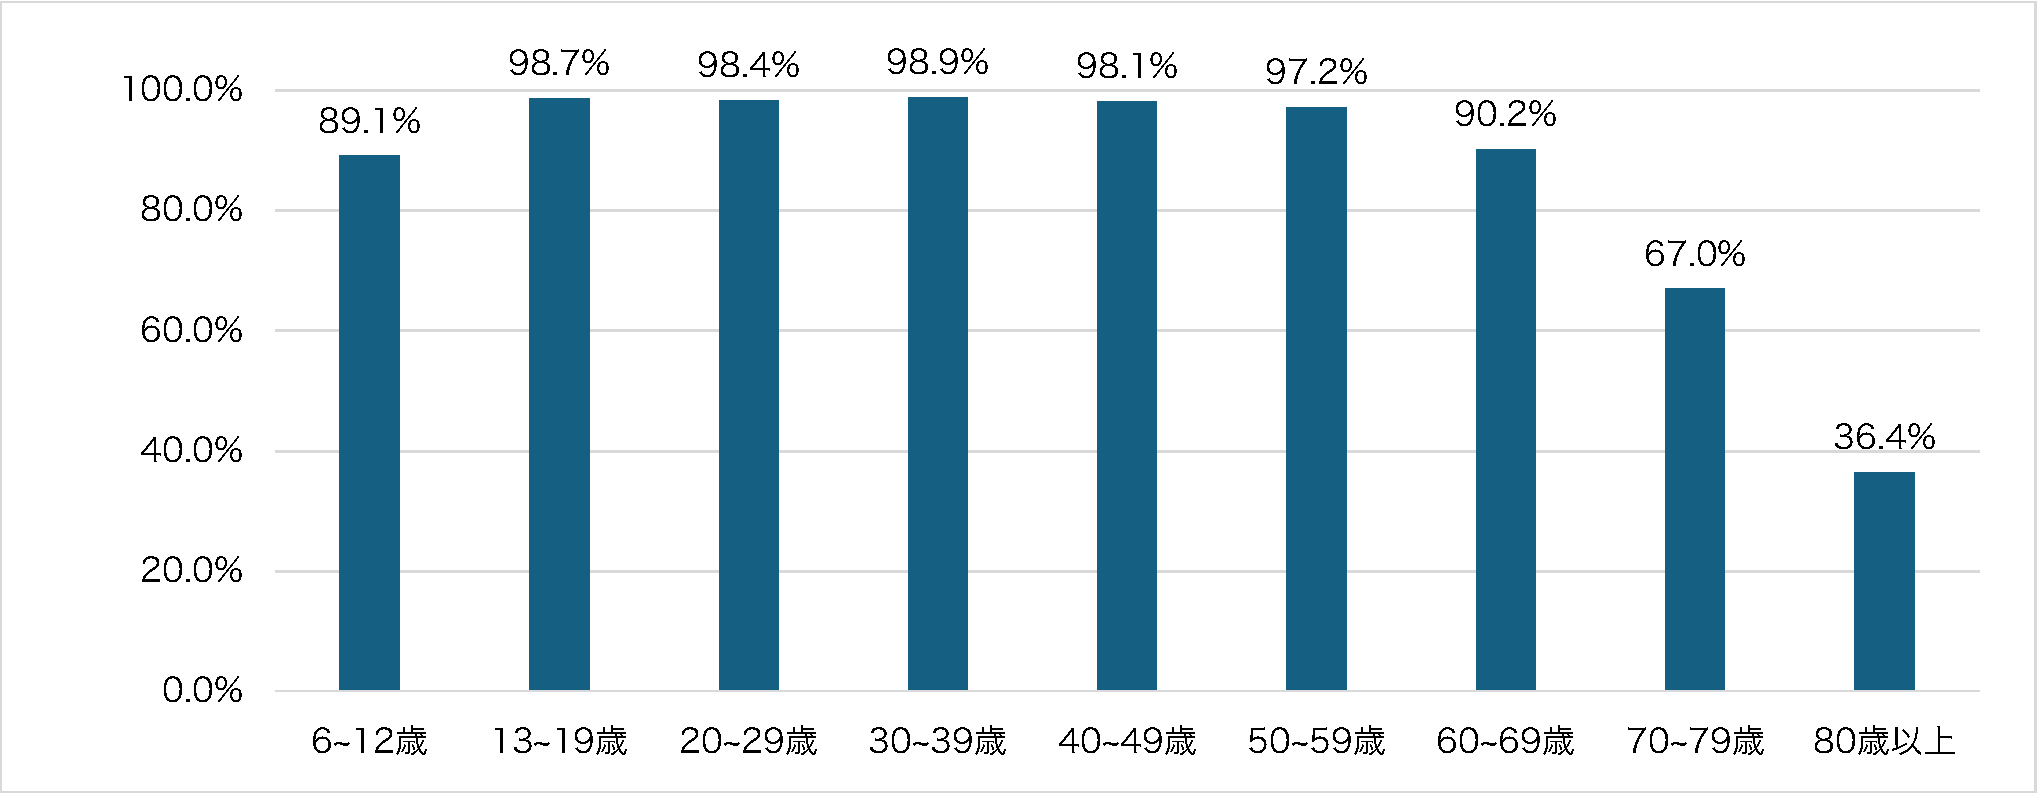
\includegraphics[width=15cm]{年代階層別.pdf}
  \caption{年代階層別インターネット利用率}
  \label{fig:nendai}
\end{figure}

%図4
\begin{figure}[!htb]
  \centering
  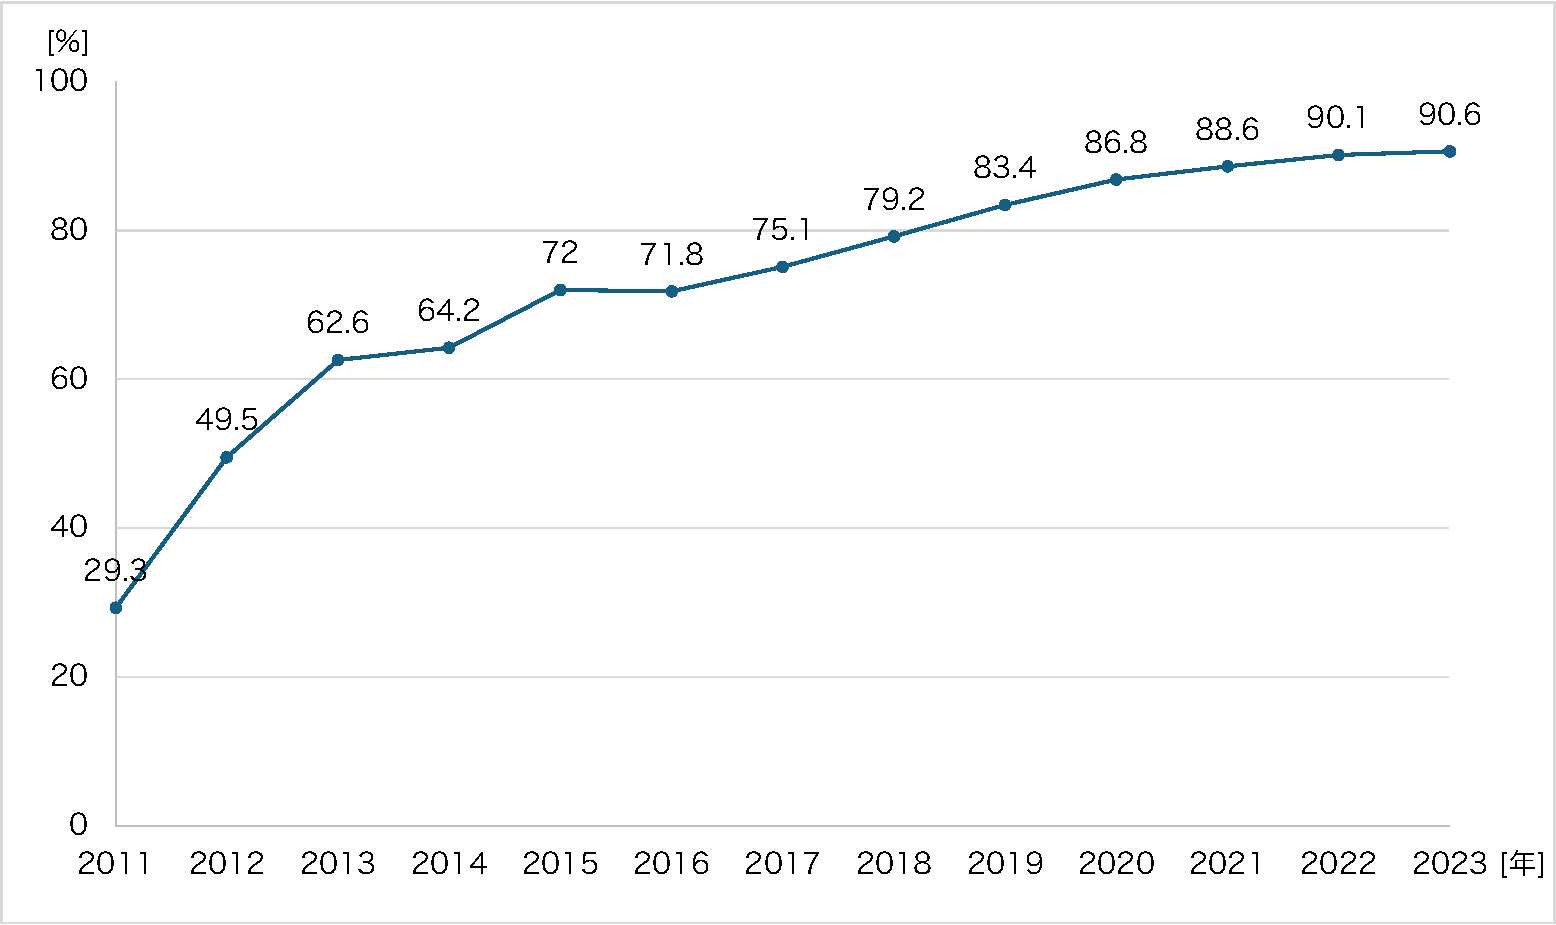
\includegraphics[width=15cm]{スマホ保持率.pdf}
  \caption{スマートフォンの保持率}
  \label{fig:sumaho}
\end{figure}

\clearpage


% 4章 2節
\subsection{生成AI}

1956年に行われたダートマス会議で「人間の脳に近い機能を持ったコンピュータープログラム」としてAI(Artificial Intelligence)という言葉が誕生し,人工知能(AI)の研究が学問分野として確立した.
第1次AIブーム(1950年後半\textasciitilde1960年代)では,特定の問題に対して解を提示する「推論」「探索」が可能になった.
第2次AIブーム(1980年代)では,「知識」を与えることで人工知能が実用可能な水準に達し,多数のエキスパートシステムが生み出された.
しかし,「知識」は人間側が直接与えなければならなかったため,世にある膨大な情報を与えるには限界があった.
第3次AIブーム(2000年\textasciitilde )では,機械学習とディープラーニングの登場により,第2次人工知能ブームの問題であった人工知能自身の知識の獲得が可能になった.
2000年代以降,AIの幅は広がり2022年からは画像や音楽などを生み出すことができる生成AIが誕生した.
生成AIの誕生を第4次AIブームとし,ChatGPTやstable diffusionなどがある\cite{soumu28}.


生成AIの1つであるChatGPTは人工知能チャットボットとして2022年12月にOpenAIが公開した.
日本では公式iOSアプリが2023年5月にリリースされ,利用率はアメリカ,インドに続いて世界で3番目となっている.
野村総合研究所ではChatGPTの利用に関する調査が行われており,2024年9月の調査では日本人の20\%が利用していることがわかった.
利用者のうち21.6\%が大学生や大学院生,専門学生であり,次に多いのが教職員で20.5\%である.
また,図\ref{fig:chat}は利用目的の調査結果であり,情報収集のほかに文章作成や要約,翻訳などに使用している人が多い\cite{nomura}.

近年ではChatGPTだけでなく,言語学習を効率化するアプリや論文や文献の要約を生成するツールなどAIを活用したアプリやツールが増えてきている.
これにより,学校などの教育現場だけでなく,学生自身が学習支援ツールとしてAIを利用する機会が多くなった.

%図5
\begin{figure}[!htb]
  \centering
  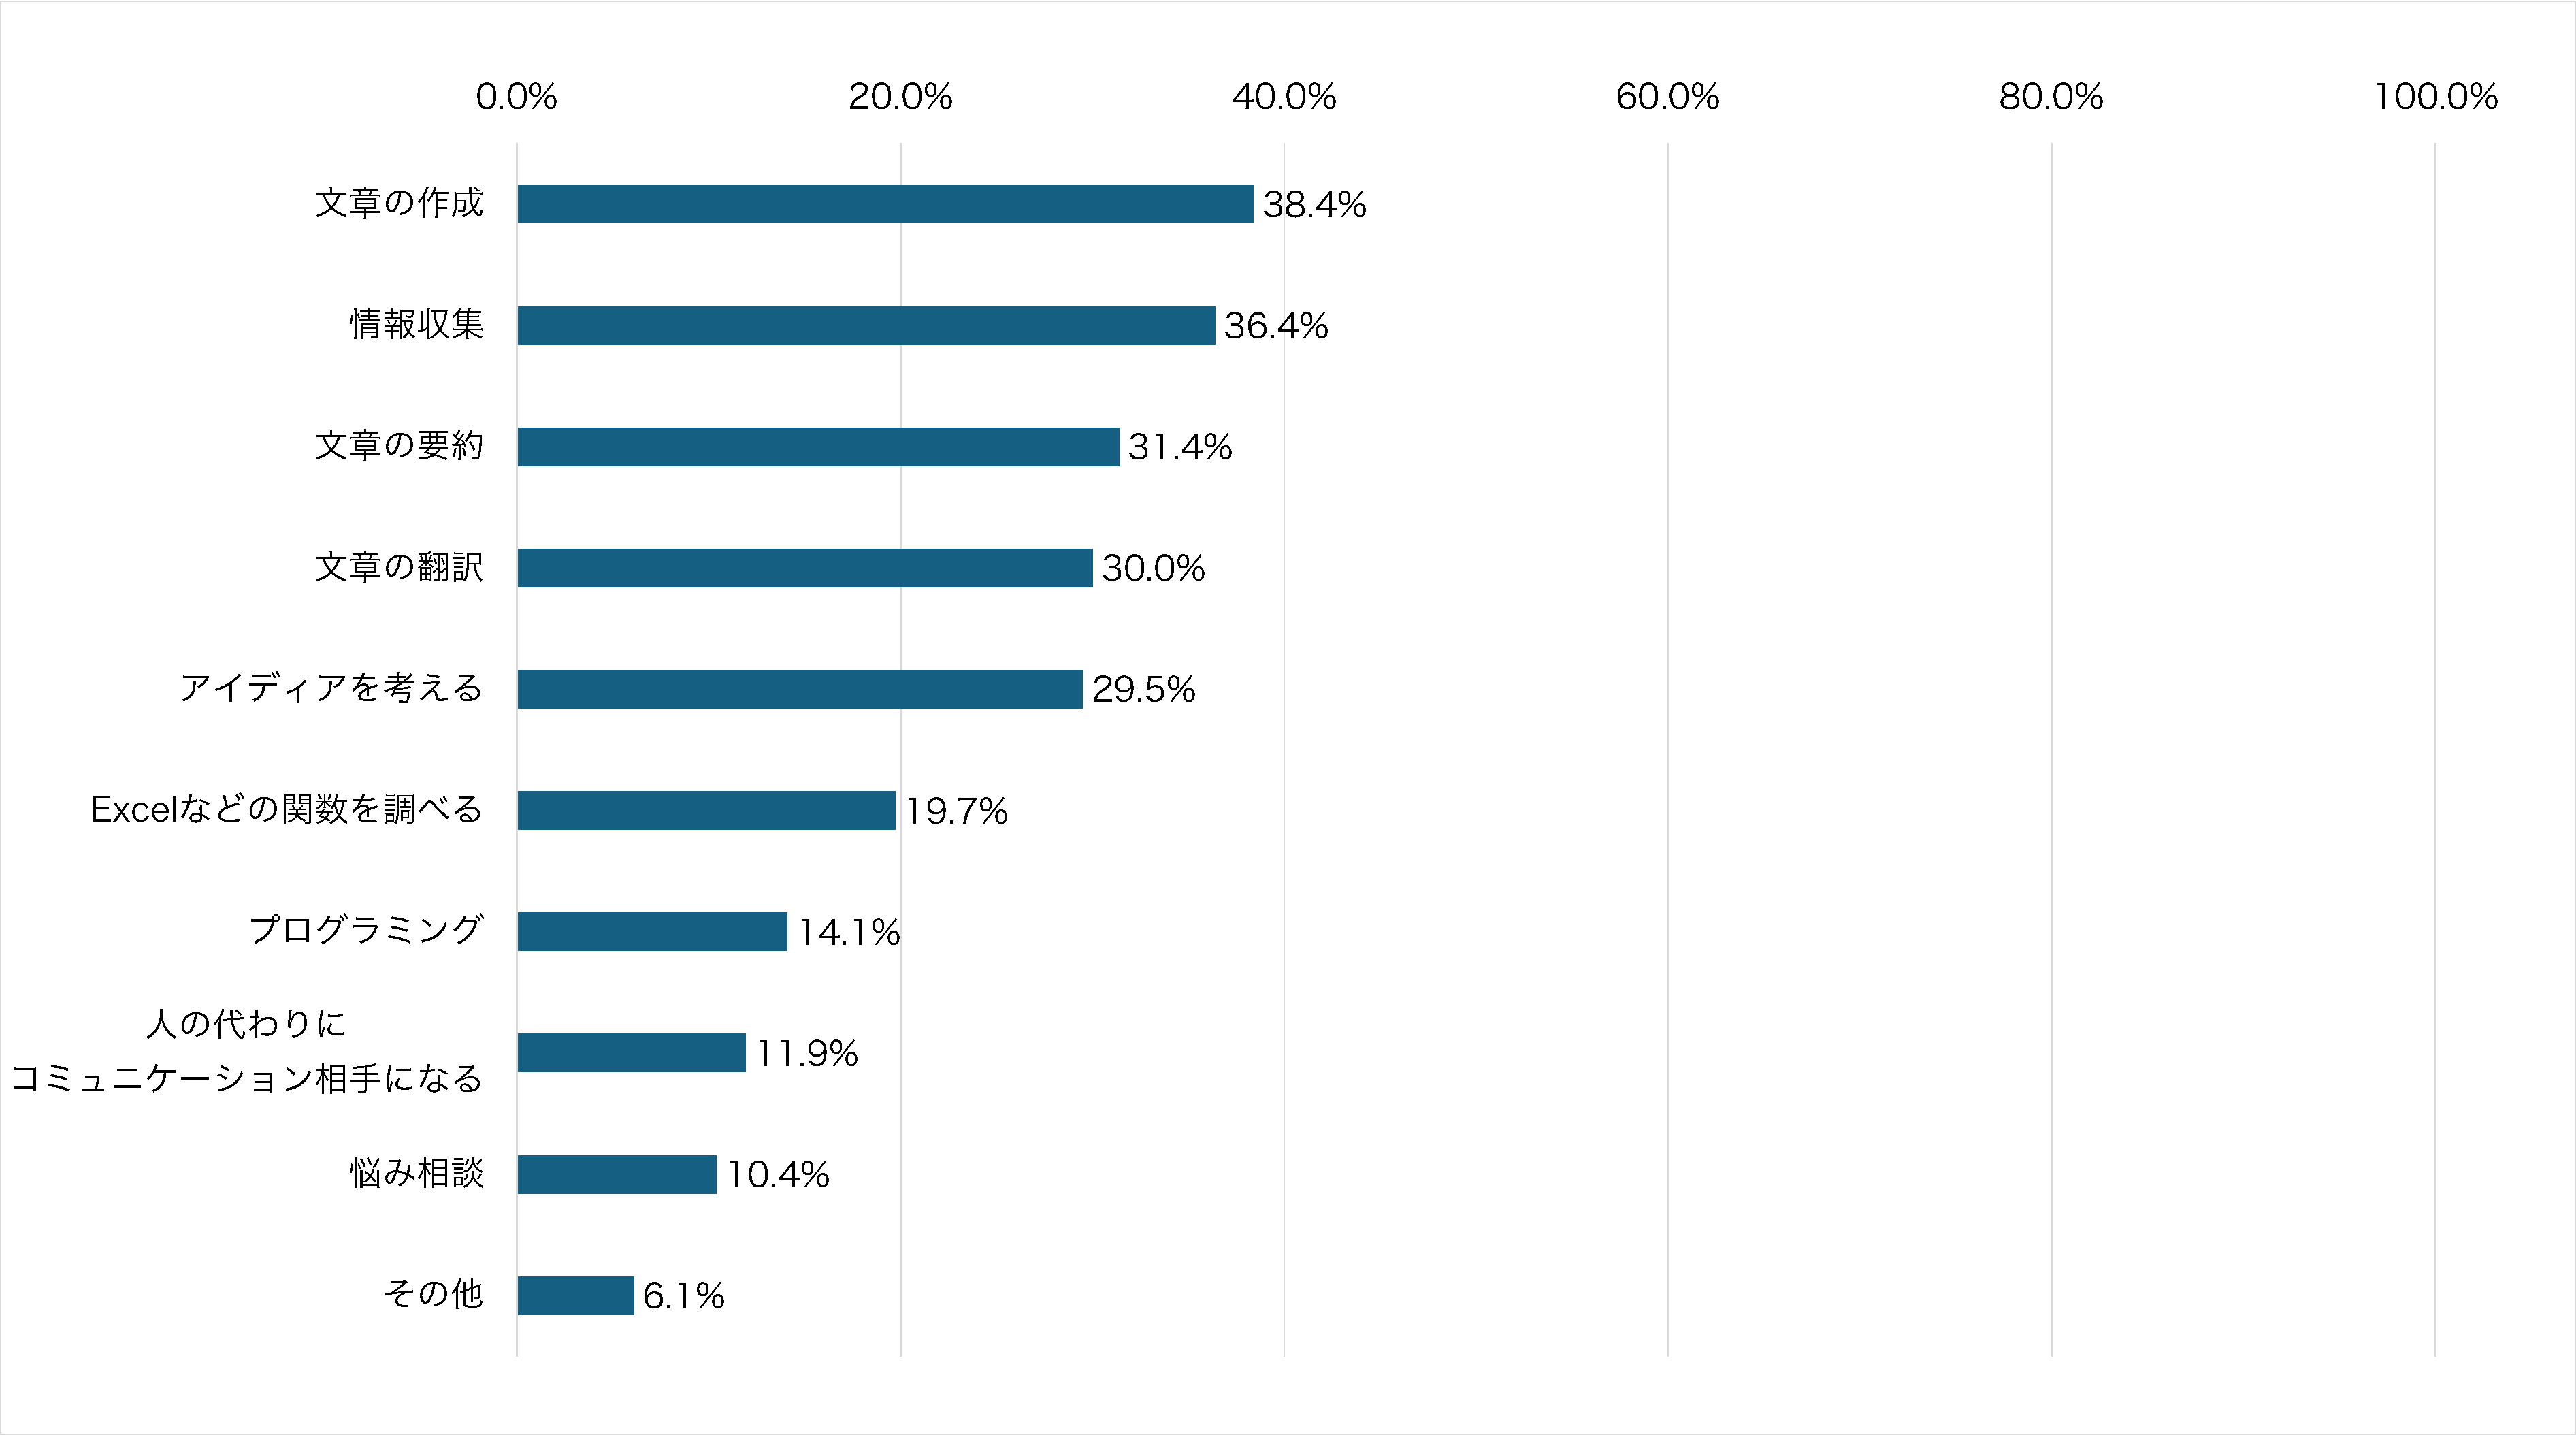
\includegraphics[width=17cm]{利用目的.pdf}
  \caption{ChatGPTの利用目的}
  \label{fig:chat}
\end{figure}

\clearpage

% 4章 3節
%\subsection{書籍}
%インターネットが普及する以前では参考書や専門書などの書籍で学生は学習をしていた.
%書籍での学習の利点として,1冊で深い知識まで学べることや知識がまとまっていることが挙げられる.
%しかし,書籍によっては内容にレベルの差があるため,自身に合ったものを選ぶのが難しいという欠点がある.

% 4章 3節
\subsection{教科書又は教員の作成した資料}
本研究では教科書は授業で扱うため書籍には含んでいない.
教科書や教員の作成した資料(以下,授業資料)は授業内で扱うため,自主学習を行う際には振り返りやすいという利点がある.
しかし,記載されている内容が限られているため,教科書や授業資料だけでは問題を解決できないという欠点がある.

% 4章 5節
%\subsection{学生ついて}
%大学では専門的な内容の学習が始まり,1,2学年では初めて扱う内容になる.
%また,3,4学年ではより専門的な知識の追求がおこなわれる.
%そのため学生はどの学年でも各科目において初学者となる.

%初学者にとって,ネット上の学習コンテンツの情報量の多さや書籍によるレベル差は大きな弱点である.
%そのため,本研究は学習する際の教材として教科書や授業資料を推奨する.

\clearpage

% 5章
\section{ネットワーク管理実習}
% 5章 1節
\subsection{概要}
ネットワーク管理実習は本校の情報科学部情報ネットワーク学科の第6セメスターで開講されている科目である.
本科目はLAN管理に必要な実践的スキルの習得を目指し,サブドメインの設計や構築を行っている.
表\ref{tb:kougi}に各週の授業内容を示す.

%表1
\begin{table}[htbp]
  \caption{ネットワーク管理実習の学習内容}
  \begin{center}
\begin{tabular}{ll}\hline
               週 & 授業内容 \\ \hline
               1 & ガイダンス\\
               2 & ユーザ管理 アクセス権\\
               3 & シェルの基本\\
               4 & TCP/IPについて\\
               5 & IPアドレッシング手法\\
               6 & ルーティングとルータ\\
               7 & パッケージのインストール\\
               8 & 名前解決の仕組み\\
               9 & DNSを利用した問い合わせの仕組み\\
              10 & DNSを利用した問い合わせの仕組み\\
              11 & メール配信の仕組み SMTPサーバの構築\\
              12 & Webサーバの構築\\
              13 & 期末テスト\\
              \hline
               \end{tabular}
               \end{center}
               \label{tb:kougi}
               \end{table}


% 5章 2節 
\subsection{Unixコマンド}
Unixは,1969年にAT\&Tのベル研究所で開発が進められたOSであり,1970年代には大学や研究所などで利用され始めた.シンプルな設計と効率性の高さから移殖・拡張が繰り返され,類似OSであるLinuxを含めてUNIX系OSと呼ばれ今でも利用されている.
Unix系OSは専用の入力画面にコマンドを打ち込んで操作するCUI方式が採用されており,ファイルの操作や情報の取得などの作業をする際に使用される.

\clearpage

% 5章 3節 
\subsection{ルーティング}
インターネットではIPアドレッシングのルールに基づき割り当てられたネットワークが互いに接続されている.
これらのネットワーク間でパケットを転送することをルーティングすると言い,ルーティングを行う装置のことをルータと呼ぶ.
ルータは隣り合うネットワーク間でパケットを中継する役割を持ち,接続するネットワークの数だけ存在する.
また,パケットを目的の宛先に届けるために多数のルータを経由するため,近接するネットワークに存在するルータブから経路を決定するためにルーティングテーブルを利用している.
ネットワーク管理実習ではルータソフトウェアFRRoutingを使用してルータの設定に必要な概念と設定手法について学習している.


% 5章 4節 
\subsection{名前解決}
デバイスに与えられているIPアドレスとFQDN(Fully Qualified Domain Name)を相互に変換することを名前解決と呼ぶ.
FQDNからIPアドレスに変換することを正引き名前解決といい,IPアドレスからFQDNに変換することを逆引き名前解決という.
ネットワーク上ではDNSサーバが名前解決を担っており,キャッシュサーバとコンテンツサーバがある.
コンテンツサーバは主に自身の所属するドメインの情報を持ち,外部へ発信している.
一方,キャッシュサーバはクライアントに代わってコンテンツサーバにドメイン情報を問い合わせる役割を持っており,高速化のために一度問い合わせた情報を一時保存している.
ネットワーク管理実習ではDNSサーバにbind9を利用し,DNSの設定を通して仕組みについて学習している.

\clearpage

% 6章 
\section{研究概要}

% 6章 1節
\subsection{授業資料}
本研究では13週にわたって行われる講義のうち4\textasciitilde10週の計7回の講義を扱って検証を行った.
表\ref{tb:kougi2}では本研究で取り扱った講義に〇をつけている.
7週目のパッケージのインストールは以前学習した内容の振り返りが中心の講義であったため,扱わなかった.
9週目と10週目の授業資料は同一のものであるため,1つの授業として扱った.
また,図\ref{fig:8no1},\ref{fig:8no2}は実際に使用されている授業資料である.
座学として仕組みなどの説明があり,実践として設定例が記載されている.

%表2
\begin{table}[htbp]
  \caption{今回扱ったネットワーク管理実習の内容}
  \begin{center}
\begin{tabular}{lll}\hline
               週 & 授業内容 & 本研究での取り扱い\\ \hline
               1 & ガイダンス & \\
               2 & ユーザ管理 アクセス権 & \\
               3 & シェルの基本 & \\
               4 & TCP/IPについて & 〇\\
               5 & IPアドレッシング手法 & 〇\\
               6 & ルーティングとルータ & 〇\\
               7 & パッケージのインストール & \\
               8 & 名前解決の仕組み & 〇\\
               9 & DNSを利用した問い合わせの仕組み & 〇\\
              10 & DNSを利用した問い合わせの仕組み & 〇\\
              11 & メール配信の仕組み SMTPサーバの構築 & \\
              12 & Webサーバの構築 & \\
              13 & テスト & \\
              \hline
               \end{tabular}
               \end{center}
               \label{tb:kougi2}
               \end{table}

\clearpage

%図6
\begin{figure}[!htb]
  \centering
  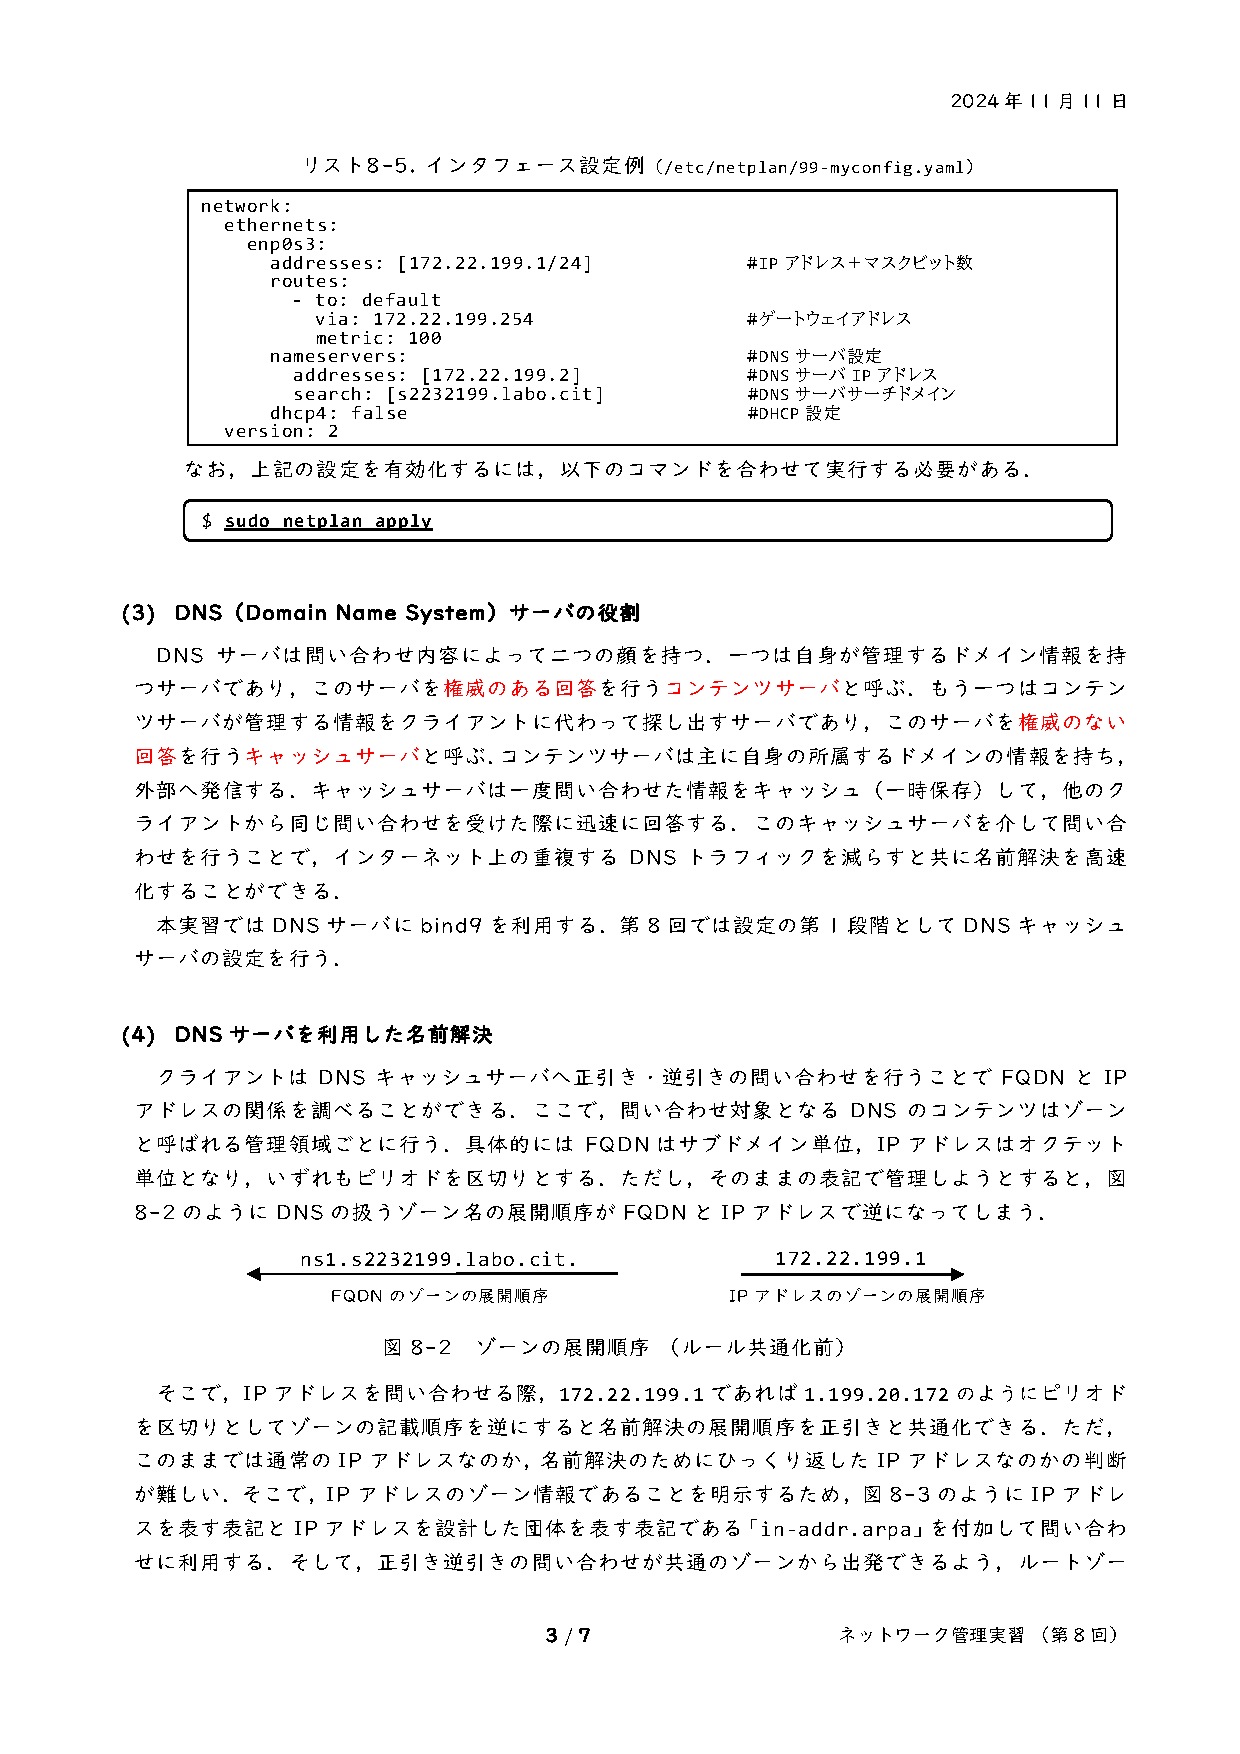
\includegraphics[width=12cm]{8週目1.pdf}
  \caption{ネットワーク管理実習 8週目授業資料(座学)}
  \label{fig:8no1}
\end{figure}

%図7
\begin{figure}[!htb]
  \centering
  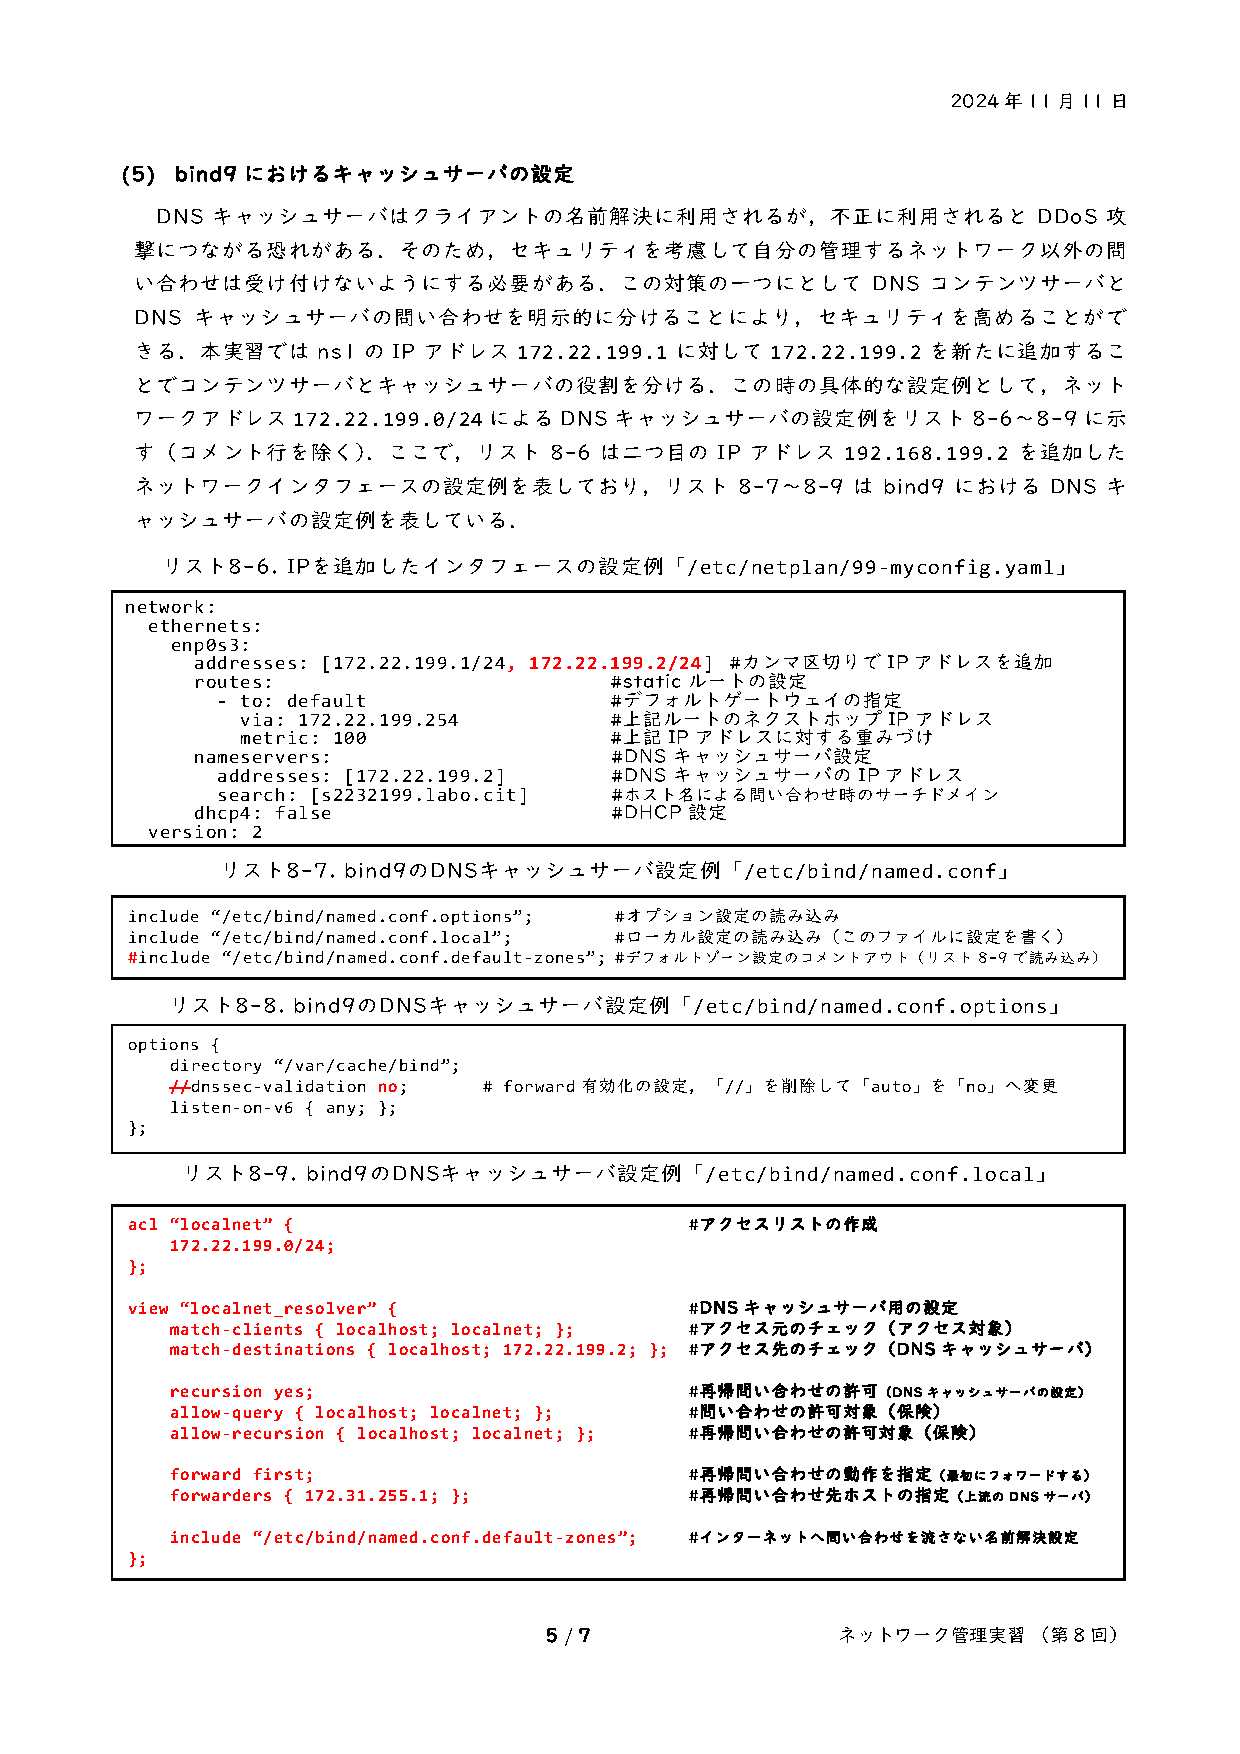
\includegraphics[width=12cm]{8週目2.pdf}
  \caption{ネットワーク管理実習 8週目授業資料(設定例)}
  \label{fig:8no2}
\end{figure}

\clearpage

% 6章 2節 
\subsection{提供するコンテンツ}
授業資料での復習が重要であるが,スマホの普及や学習意欲の観点から学習する際にネット上のコンテンツを利用している.
このような実態となってしまう原因として,現在使用している授業資料は文字が多く,専門用語が並ぶため学生が学習を始めるには抵抗を持ちやすくなっていることが考えられる.
加えて,電子資料として配布されているため,スマホで見るには小さく,パソコンで見るには場所を選ばなければならない.

そこで本研究では授業資料での復習を促すために学生が扱いやすい要素を取り入れ,学習への抵抗を解消できるようなコンテンツを提供する.
扱いやすい要素として,短時間でどこでも使用できることを重要視し,学生が扱いなれているスマートフォンで利用できる1\textasciitilde3分程度の動画コンテンツを提供した.
動画内では文字ではなく図や表を用いた説明を行い,小さい画面でも見やすいような設計にした.
また,授業資料に促すという観点からは,理解に難しい内容の簡単な解説や授業の前提となる知識,授業内容が深くできるような内容を取り入れるだけでなく,授業資料と結び付けやすいように動画内に対応しているページ番号を記載した.


%本研究で提供するコンテンツは扱いやすさと授業資料に促せるような要素を取り入れ,補助教材として成り立つように設計した.
%扱いやすさの観点では,学習に抵抗を持たせないように短時間でどこでも使用できることを重要視した.
%これらのことから,本研究では学生が扱いなれているスマートフォンで利用できる1\textasciitilde3分程度の動画コンテンツを提供した.
%また,授業資料に促す言う観点からは,理解の難しい内容の簡単な解説や授業の前提となる知識,授業内容の深堀だけでなく,授業資料と結び付けやすいように動画内に対応しているページ番号を記載した.

%扱いやすさという観点から,学生が普段から使用しているスマホで利用できるコンテンツとして動画形式を採用した.
%動画コンテンツは学生が抵抗なく見れるように1\textasciitilde3分のショート動画として提供した.

%授業資料に促すという観点から,提案した動画コンテンツには理解の難しい内容の簡単な解説や授業の前提となる知識,授業の深堀など授業資料の補助として成り立つような内容を取り入れた.
%また,授業資料と結び付けやすいように動画内に対応しているページ番号を記載した.

動画コンテンツの作成にはゆっくりムービーメーカーとVOICEVOXを使用し,毎週YouTubeでプレイリストを作成して公開した.

\clearpage

% 7章
\section{事前調査}
% 7章 1節
\subsection{概要}
学生がどのような学習を行っているか調査するため,本学の情報科学部情報ネットワーク学科で開講されているネットワーク管理実習を受講している学生を対象に調査を行い,〇〇名から回答を得た.


% 7章 2節
\subsection{アンケート項目}
学習調査に関するアンケートは動画コンテンツを提供する前に行った.
アンケートの質問項目を表\ref{tb:anke1}に示す.
時間に関する質問を2問,学習する際の状況についての質問を2問の計4問を選択式で用意した.

%表3
\begin{table}[htbp]
  \caption{学習状況に関するアンケート}
  \begin{center}
\begin{tabular}{ll}\hline
               番号 & 質問 \\ \hline
               問1 & 1週間の1つの演習授業に関する学習時間\\
               問2 & 1週間のスマホの利用時間\\
               問3 & 授業でわからない時の解決方法について教えてください\\
               問4 & スマホを用いて学習する際に利用するものについて教えてください\\
              \hline
               \end{tabular}
               \end{center}
               \label{tb:anke1}
               \end{table}


\clearpage

% 7章 3節
\subsection{アンケート結果 問1}
テスト1週間前とテスト期間外の2つに分けた「問1.1週間の1つの演習授業に関する学習時間」という質問では表\ref{tb:anke1_1}の選択肢を設けた.
その結果を図\ref{fig:benkyo}に示す.
テスト1週間前ではほとんどの学生が1-3時間以上の学習を行っているのに対し,テスト期間外では80\%以上の学生が1時間以下の学習時間であることがわかった.
これらのことからテストのためだけの学習になっており,身についていないと考えられる.

%表4
\begin{table}[htbp]
  \caption{問1の選択肢}
  \begin{center}
\begin{tabular}{ll}\hline
               選択肢 & 学習時間 \\ \hline
               1 & 30分未満\\
               2 & 30分\textasciitilde1時間\\
               3 & 1\textasciitilde3時間\\
               4 & 3\textasciitilde5時間\\
               5 & 5時間以上\\
              \hline
               \end{tabular}
               \end{center}
               \label{tb:anke1_1}
               \end{table}

%図8
\begin{figure}[!htb]
  \centering
  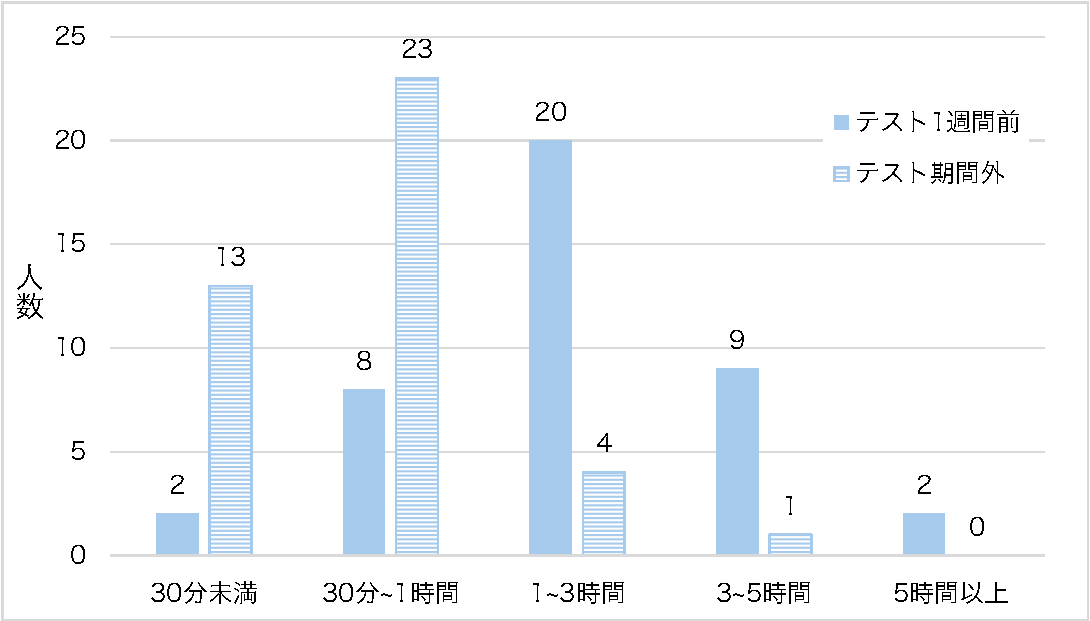
\includegraphics[width=15cm]{学習時間.pdf}
  \caption{テスト1週間前とテスト期間外の学習時間}
  \label{fig:benkyo}
\end{figure}

\clearpage

%7章 4節
\subsection{アンケート結果 問2}
「問2.1週間のスマホの利用時間」という質問ではSNS,動画サイト,ゲーム,漫画アプリの4項目で表\ref{tb:anke1_2}の選択肢を設けた.
その結果を図\ref{fig:sns},\ref{fig:douga},\ref{fig:game},\ref{fig:manga}に示す.
最も利用時間が多いのは動画コンテンツであり,ほとんどの学生が1週間に3時間以上見ていることがわかった.
また,漫画アプリ以外の項目では半分の学生が1時間以上利用しており,1週間でのスマホの利用時間が長いことがわかった.

%表5
\begin{table}[htbp]
  \caption{問2の選択肢}
  \begin{center}
\begin{tabular}{ll}\hline
               選択肢 & 利用時間 \\ \hline
               1 & 30分未満\\
               2 & 30分\textasciitilde1時間\\
               3 & 1\textasciitilde3時間\\
               4 & 3\textasciitilde5時間\\
               5 & 5時間以上\\
              \hline
               \end{tabular}
               \end{center}
               \label{tb:anke1_2}
               \end{table}
\clearpage

%図9~12
\begin{figure}[!htb]
\centering
\begin{minipage}[b]{0.49\columnwidth}
    \centering
    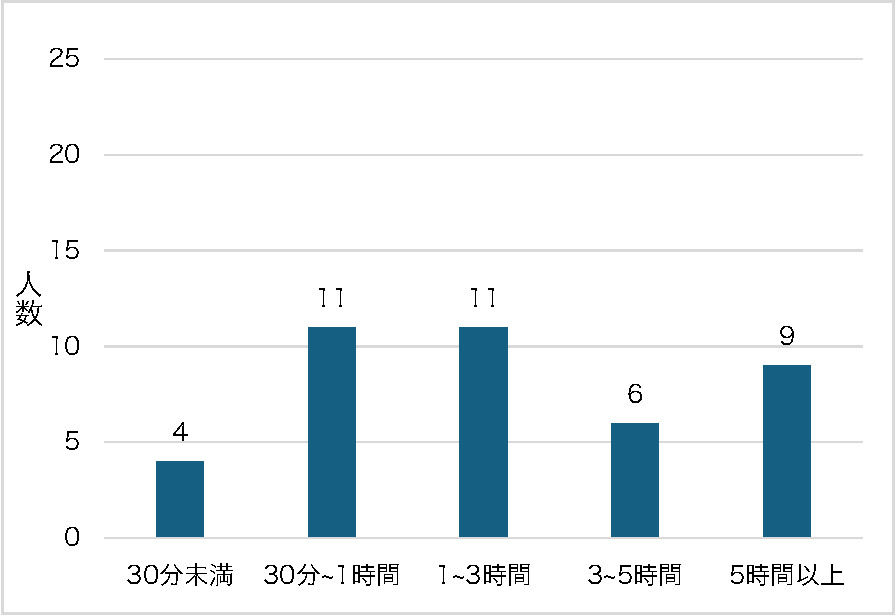
\includegraphics[width=1.0\columnwidth]{SNS.pdf}
    \caption{SNS}
    \label{fig:sns}
\end{minipage}
\begin{minipage}[b]{0.49\columnwidth}
    \centering
    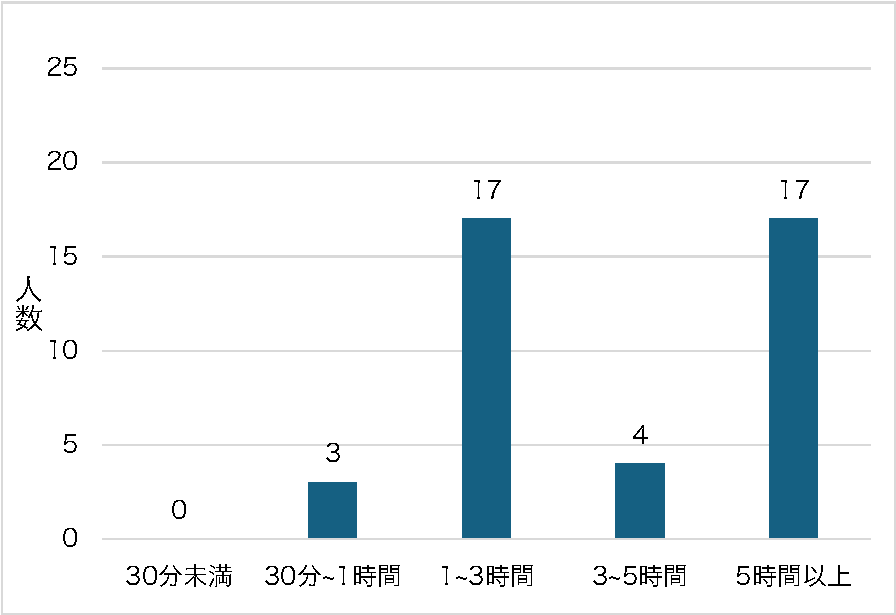
\includegraphics[width=1.0\columnwidth]{動画サイト使用時間.pdf}
    \caption{動画サイト}
    \label{fig:douga}
\end{minipage}
\end{figure}

\begin{figure}[!htb]
\centering
\begin{minipage}[b]{0.49\columnwidth}
    \centering
    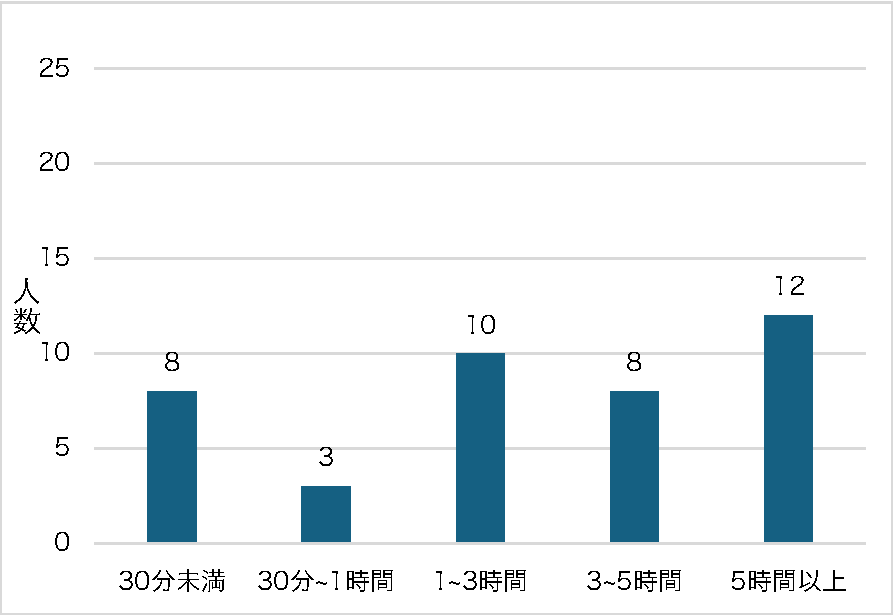
\includegraphics[width=1.0\columnwidth]{ゲーム.pdf}
    \caption{ゲーム}
    \label{fig:game}
\end{minipage}
\begin{minipage}[b]{0.49\columnwidth}
    \centering
    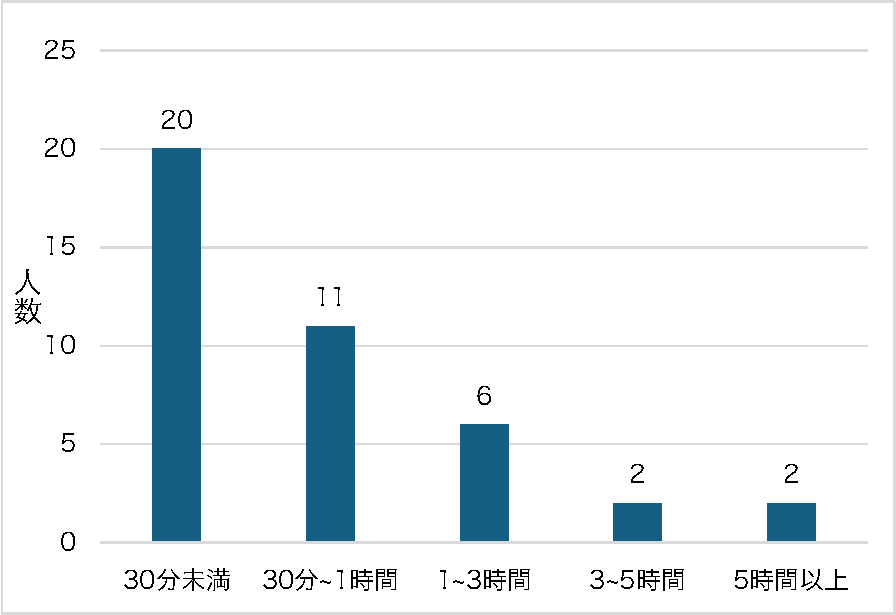
\includegraphics[width=1.0\columnwidth]{漫画アプリ.pdf}
    \caption{漫画アプリ}
    \label{fig:manga}
\end{minipage}
\end{figure}

\clearpage

%7章 5節
\subsection{アンケート結果 問3}
「問3.授業でわからない時の解決方法」という質問ではスマホ/PCで調べる,本を借りる,先生に聞く,友達に聞くの4項目で表\ref{tb:anke1_3}の選択肢を設けた.
その結果を図\ref{fig:pc},\ref{fig:hon},\ref{fig:sensei},\ref{fig:friends}に示す.
「スマホ/PCで調べる」という項目では90\%の学生がよく使うと回答した.
一方で「本を借りて調べる」という項目では使わない,又はあまり使わないと回答した学生が70\%を超えている.
また,よく使うと回答した学生の割合は「先生に聞く」より「友達に聞く」という項目の方が高いことから,身近なもので解決するようになっていると考えられる.

%表6
\begin{table}[htbp]
  \caption{問3の選択肢}
  \begin{center}
\begin{tabular}{ll}\hline
選択肢 & 項目\\ \hline
               1 & よく使う \\ 
               2 & たまに使う\\
               3 & あまり使わない\\
               4 & 使わない\\
              \hline
               \end{tabular}
               \end{center}
               \label{tb:anke1_3}
               \end{table}

\clearpage

%図13~16
\begin{figure}[!htb]
\centering
\begin{minipage}[b]{0.49\columnwidth}
    \centering
    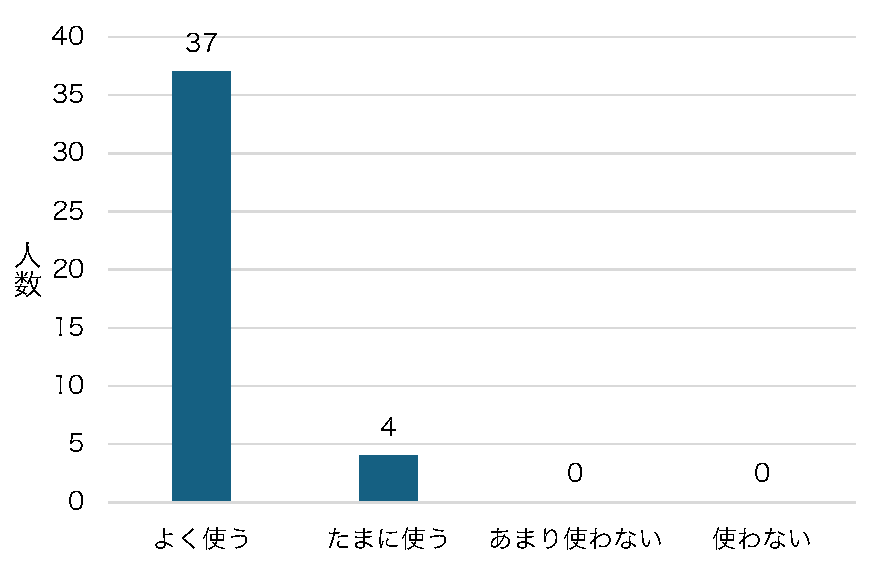
\includegraphics[width=1.0\columnwidth]{スマホPCで調べる.pdf}
    \caption{スマホ/PCで調べる}
    \label{fig:pc}
\end{minipage}
\begin{minipage}[b]{0.49\columnwidth}
    \centering
    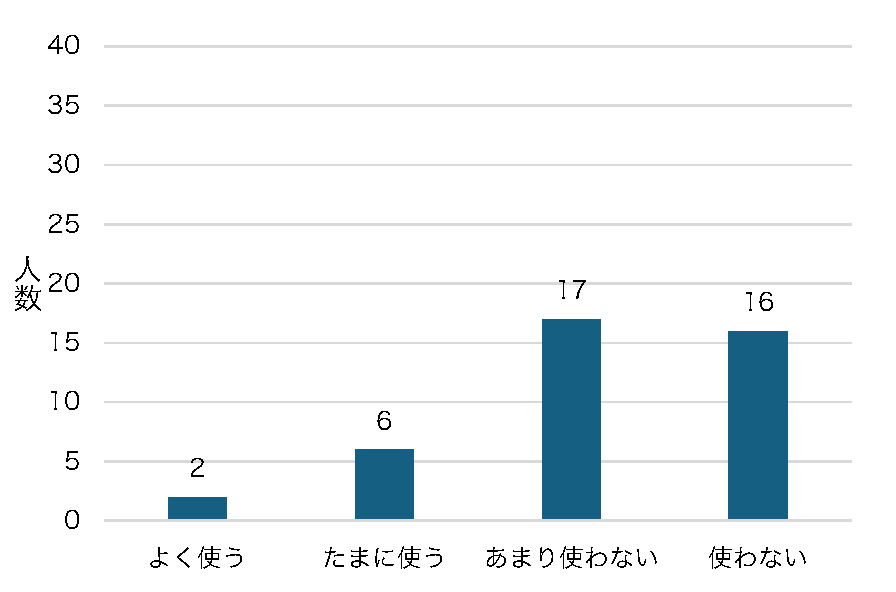
\includegraphics[width=1.0\columnwidth]{本を借りる.pdf}
    \caption{本を借りる}
    \label{fig:hon}
\end{minipage}
\end{figure}

\begin{figure}[!htb]
\centering
\begin{minipage}[b]{0.49\columnwidth}
    \centering
    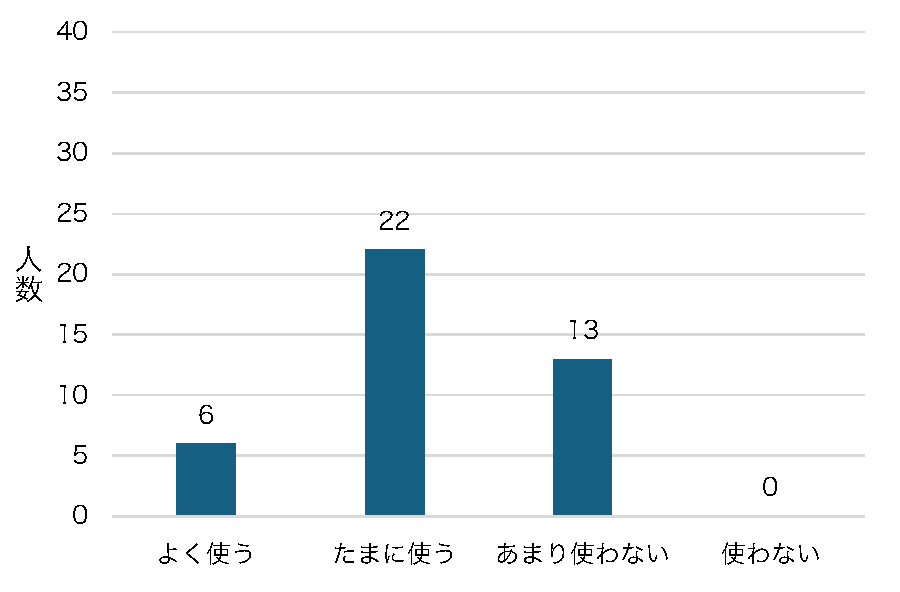
\includegraphics[width=1.0\columnwidth]{先生に聞く.pdf}
    \caption{先生に聞く}
    \label{fig:sensei}
\end{minipage}
\begin{minipage}[b]{0.49\columnwidth}
    \centering
    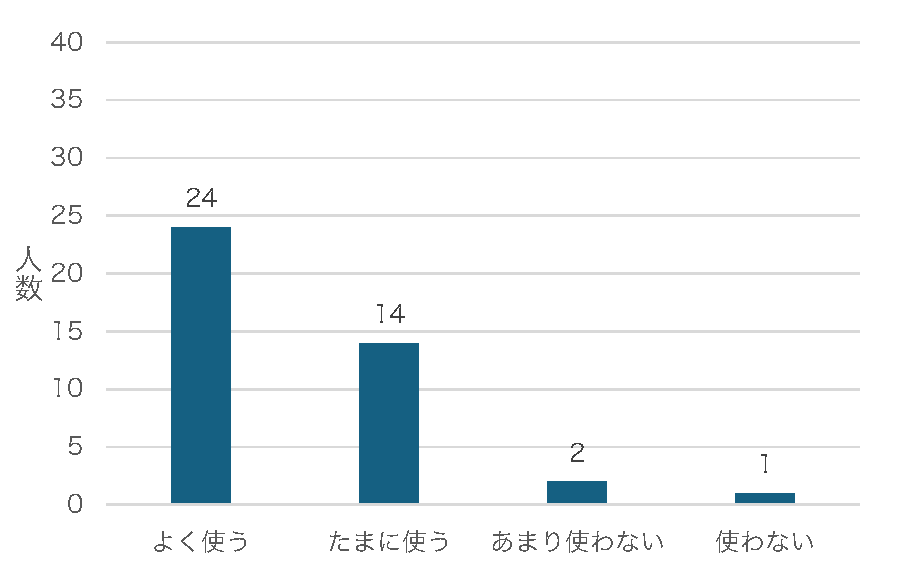
\includegraphics[width=1.0\columnwidth]{友達に聞く.pdf}
    \caption{友達に聞く}
    \label{fig:friends}
\end{minipage}
\end{figure}

\clearpage

%7章 6節
\subsection{アンケート結果 問4}
「問4.スマホを用いて学習する際に利用するもの」という質問では検索,動画サイト,ChatGPT,学習コミュニティの4項目で表\ref{tb:anke1_4}の選択肢を設けた.
その結果を図\ref{fig:kensaku},\ref{fig:dougasaito},\ref{fig:ChatGPT2},\ref{fig:community}に示す.
90\%以上の学生が検索を使っており,学習コミュニティの利用は少ないことがわかる.
また,近年AIが発達したことでChatGPTを利用している学生も多く,よく利用していると回答した学生は動画サイトと変わらないことがわかった.

%表7
\begin{table}[htbp]
  \caption{問4の選択肢}
  \begin{center}
\begin{tabular}{ll}\hline
選択肢 & 項目\\ \hline
               1 & よく使う \\ 
               2 & たまに使う\\
               3 & あまり使わない\\
               4 & 使わない\\
              \hline
               \end{tabular}
               \end{center}
               \label{tb:anke1_4}
               \end{table}

\clearpage

%図17~20
\begin{figure}[!htb]
\centering
\begin{minipage}[b]{0.49\columnwidth}
    \centering
    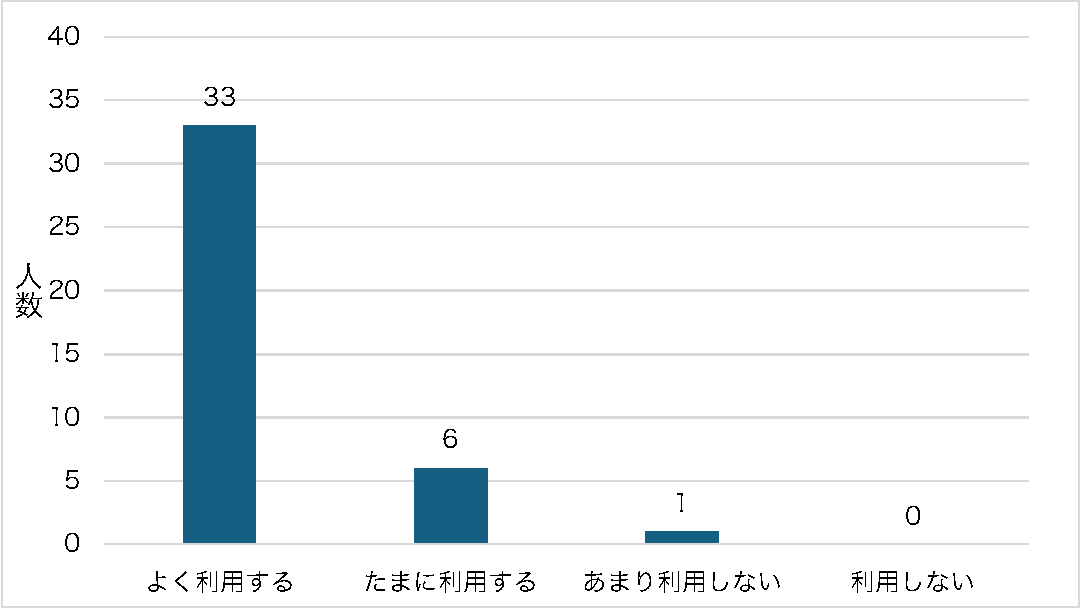
\includegraphics[width=1.0\columnwidth]{検索.pdf}
    \caption{検索}
    \label{fig:kensaku}
\end{minipage}
\begin{minipage}[b]{0.49\columnwidth}
    \centering
    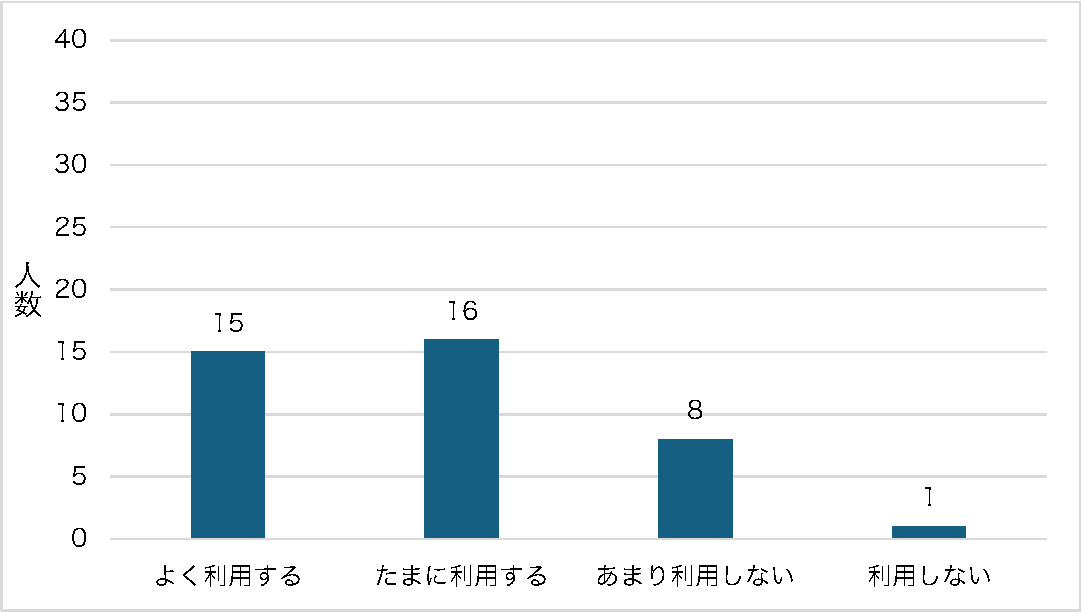
\includegraphics[width=1.0\columnwidth]{動画サイト.pdf}
    \caption{動画サイト}
    \label{fig:dougasaito}
\end{minipage}
\end{figure}

\begin{figure}[!htb]
\centering
\begin{minipage}[b]{0.49\columnwidth}
    \centering
    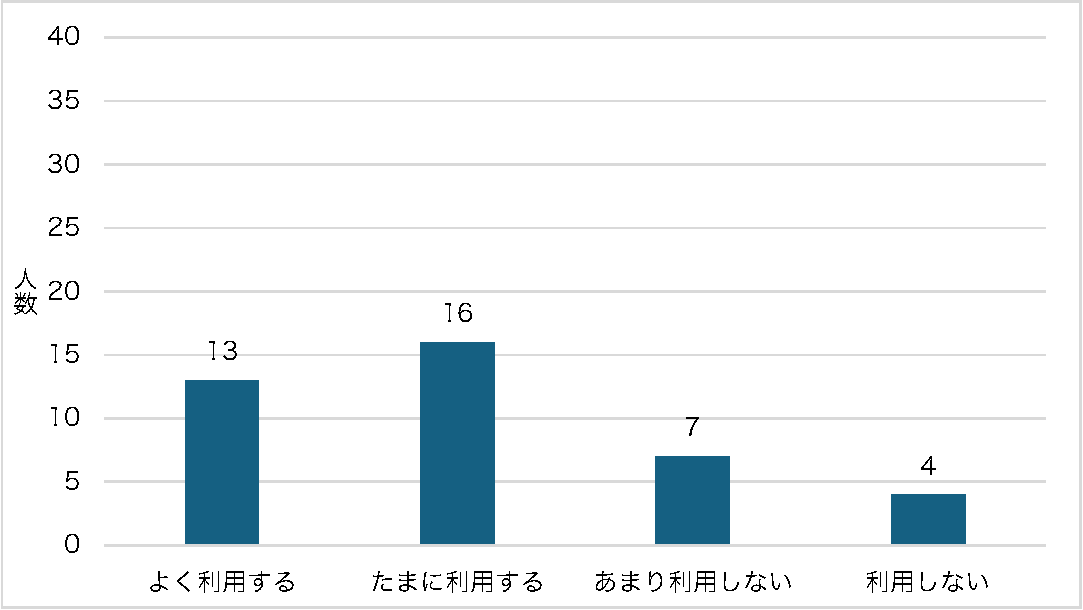
\includegraphics[width=1.0\columnwidth]{ChatGPT.pdf}
    \caption{ChatGPT}
    \label{fig:ChatGPT2}
\end{minipage}
\begin{minipage}[b]{0.49\columnwidth}
    \centering
    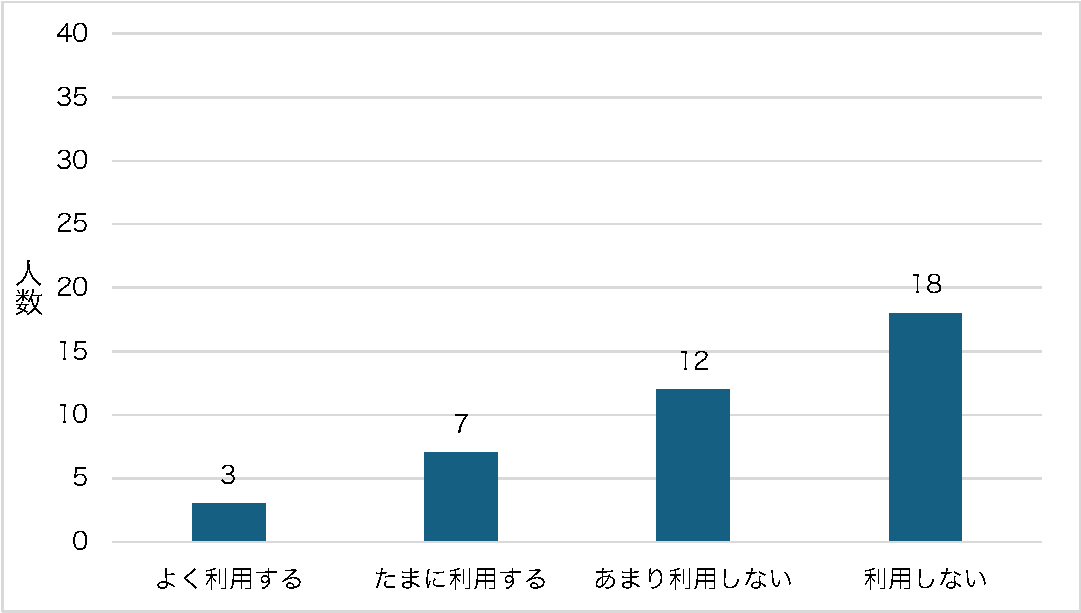
\includegraphics[width=1.0\columnwidth]{学習コミュニティ.pdf}
    \caption{学習コミュニティ}
    \label{fig:community}
\end{minipage}
\end{figure}

\clearpage


% 8章
\section{コンテンツ評価}
% 8章 1
\subsection{概要}
本学の情報科学部情報ネットワーク学科で開講されているネットワーク管理実習を受講している学生に動画コンテンツを提供し,評価を行った.
アンケートでは〇〇名から回答を得た.


% 8章 2
\subsection{アンケート項目}

% 8章 2 1
\subsubsection{学習時間に関するアンケート項目}
問1\textasciitilde3では,授業資料を用いた学習時間とコンテンツの利用による授業資料での学習時間を比較して,コンテンツの有効性について調査した.
動画視聴回数の質問1問と授業資料を用いた学習時間と動画を経由して学習した時間の質問を2問用意した.
アンケートの質問項目を表\ref{tb:anke2}に示す.

%表8
\begin{table}[htbp]
  \caption{授業資料での学習}
  \begin{center}
\begin{tabular}{ll}\hline
               番号 & 質問 \\ \hline
               問1 & manabaで提供した動画コンテンツの視聴回数を教えてください\\
               問2 & 授業資料(manabaで配布しているPDF資料)を用いてどのくらい勉強しましたか\\
               問3 & 授業資料を用いた学習のうち,manabaで紹介したコンテンツを経由したのはどのくらいですか\\
              \hline
               \end{tabular}
               \end{center}
               \label{tb:anke2}
               \end{table}

\clearpage

% 8章 2 2
\subsubsection{学習への関心に関するアンケート項目}
「問1.manabaで提供した動画コンテンツの視聴回数を教えてください」という質問に表\ref{tb:anke2_0}の選択肢を用意し,選択肢1,2を回答した学生を対象に学生の学習に対する関心について調査した.
質問項目を表\ref{tb:anke2_1}に示す.

%表9
\begin{table}[htbp]
  \caption{問1の選択肢}
  \begin{center}
\begin{tabular}{ll}\hline
選択肢 & 回数\\ \hline
               1 & 0回\\
               2 & 1\textasciitilde3回\\
               3 & 4\textasciitilde6回\\
               4 & 7回以上\\
               \hline
                \end{tabular}
                \end{center}
                \label{tb:anke2_0}
                \end{table}

%表10                
\begin{table}[htbp]
  \caption{視聴回数が少ない理由}
  \begin{center}
\begin{tabular}{ll}\hline
               番号 & 質問 \\ \hline
               問4 & 視聴しなかったもしくは,視聴回数が少ない理由を教えてください\\
               問5 & その他の理由を教えてください\\
              \hline
               \end{tabular}
               \end{center}
               \label{tb:anke2_1}
               \end{table}


% 8章 2 3
\subsubsection{提供した動画コンテンツの形式に関するアンケート項目}
「8.2.2 学習への関心に関するアンケート項目」で使用した表\ref{tb:anke2_0}の選択肢のうち,選択肢3,4に回答した学生を対象に提供した動画コンテンツについて調査した.
質問項目を表\ref{tb:anke2_2}に示す.

%表11
\begin{table}[htbp]
  \caption{提供した動画コンテンツの評価}
  \begin{center}
\begin{tabular}{ll}\hline
               番号 & 質問 \\ \hline
               問4 & 授業資料の振り返りとして有効でしたか\\
               問5 & 学習コンテンツとして動画の形式は適切だと思いますか\\
               問6 & プレイリストのような工夫は有効だと思いますか\\
               問7 & 提供した動画の時間(1\textasciitilde3分程度)は適切でしたか\\
              \hline
               \end{tabular}
               \end{center}
               \label{tb:anke2_2}
               \end{table}

\clearpage


% 8章 2 4
\subsubsection{学習ツールに関するアンケート項目}
学生が自主学習をする際に利用した学習ツールについて各授業ごとに選択肢を用意し,調査した.
質問項目を表\ref{tb:anke2_3}に示す.

%表12
\begin{table}[htbp]
  \caption{各授業ごとに利用した学習ツール}
  \begin{center}
\begin{tabular}{ll}\hline
               番号 & 質問 \\ \hline
               問1 & 4回目(TCP/IP)について\\
               問2 & 5回目(IPアドレッシング手法)について\\
               問3 & 6回目(ルーティングとルータ)について\\
               問4 & 8回目(名前解決の仕組み)について\\
               問5 & 9,10回目(DNSを利用した問い合わせの仕組み)について\\
              \hline
               \end{tabular}
               \end{center}
               \label{tb:anke2_3}
               \end{table}

\clearpage

% 8章 3
\subsection{アンケート結果による考察}

% 8章 3 1
\subsubsection{学習時間に関する考察}
「問1.manabaで提供した動画コンテンツの視聴回数を教えてください」という質問の回答結果で比較し,学習時間について考察した.
図\ref{fig:sityou}は視聴回数別の人数である.

%図21
\begin{figure}[!htb]
  \centering
  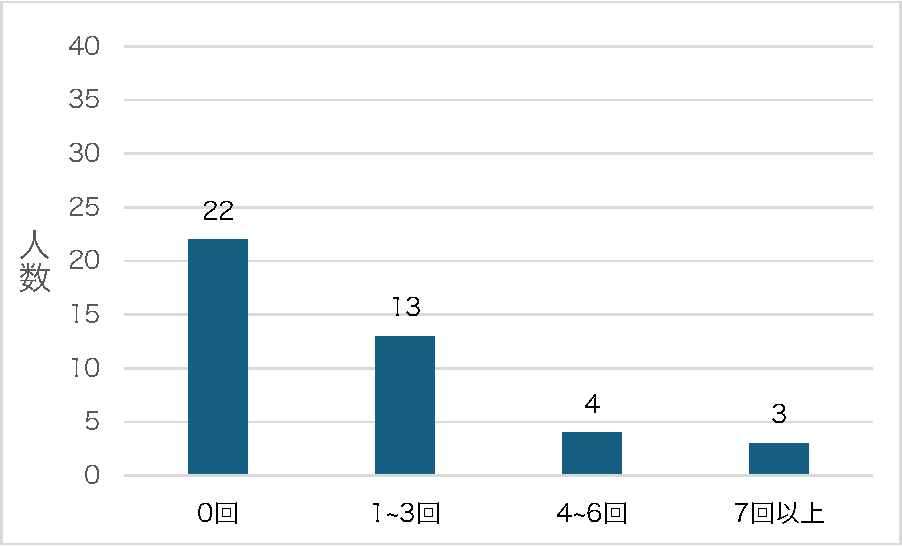
\includegraphics[width=15cm]{動画の視聴回数.pdf}
  \caption{動画の視聴回数}
  \label{fig:sityou}
\end{figure}

「問2.授業資料(manabaで配布しているPDF資料)を用いてどのくらい勉強しましたか」「問3.授業資料を用いた学習のうち,manabaで紹介したコンテンツを経由したのはどのくらいですか」という質問にそれぞれ表\ref{tb:anke2_8}の選択肢を設け.視聴回数別に学習時間を比較した.
その結果を図\ref{fig:jikan},\ref{fig:jikan2}に示す.
図\ref{fig:jikan}より,授業資料による学習時間が30分未満の学生が多く,視聴時間別で学習時間の差は見られなかった.
図\ref{fig:jikan2}では提供した動画コンテンツを経由して学習した学生が少なく,学習時間の減少に対して効果がなかったことがわかる.
また,視聴回数が1回以上の学生のグラフから,動画コンテンツを視聴したにもかかわらず授業資料に促せなかった理由としてコンテンツ内容に問題があったと考えられる.

%表13
\begin{table}[htbp]
  \caption{問1の選択肢}
  \begin{center}
\begin{tabular}{ll}\hline
選択肢 & 学習時間\\ \hline
               1 & 30分未満\\
               2 & 30分\textasciitilde1時間\\
               3 & 1\textasciitilde3時間\\
               4 & 3\textasciitilde5時間\\
               5 & 5時間以上\\
               \hline
                \end{tabular}
                \end{center}
                \label{tb:anke2_8}
                \end{table}

%図22
\begin{figure}[!htb]
  \centering
  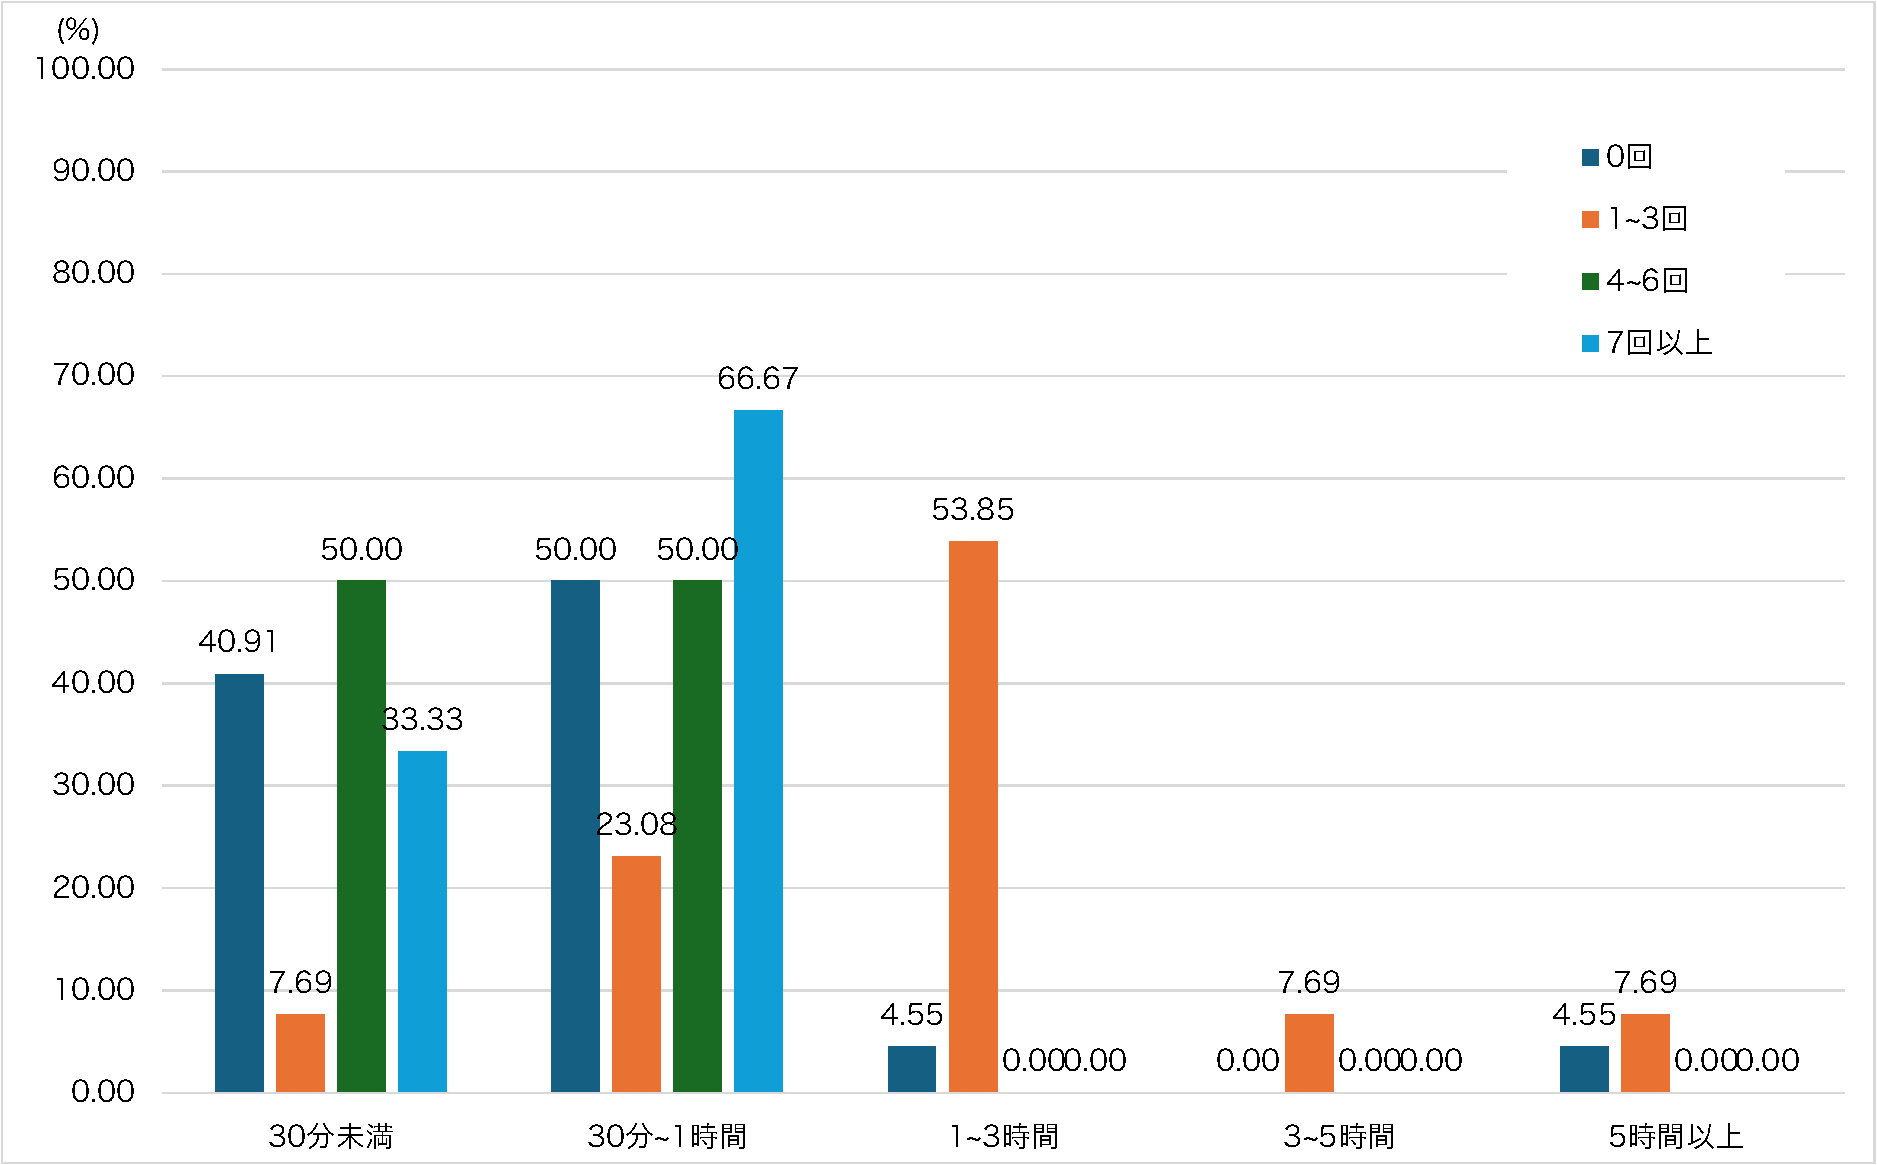
\includegraphics[width=15cm]{視聴回数別学習時間.pdf}
  \caption{視聴回数別の学習時間(問1,問2より)}
  \label{fig:jikan}
\end{figure}

%図23 図の変更
\begin{figure}[!htb]
  \centering
  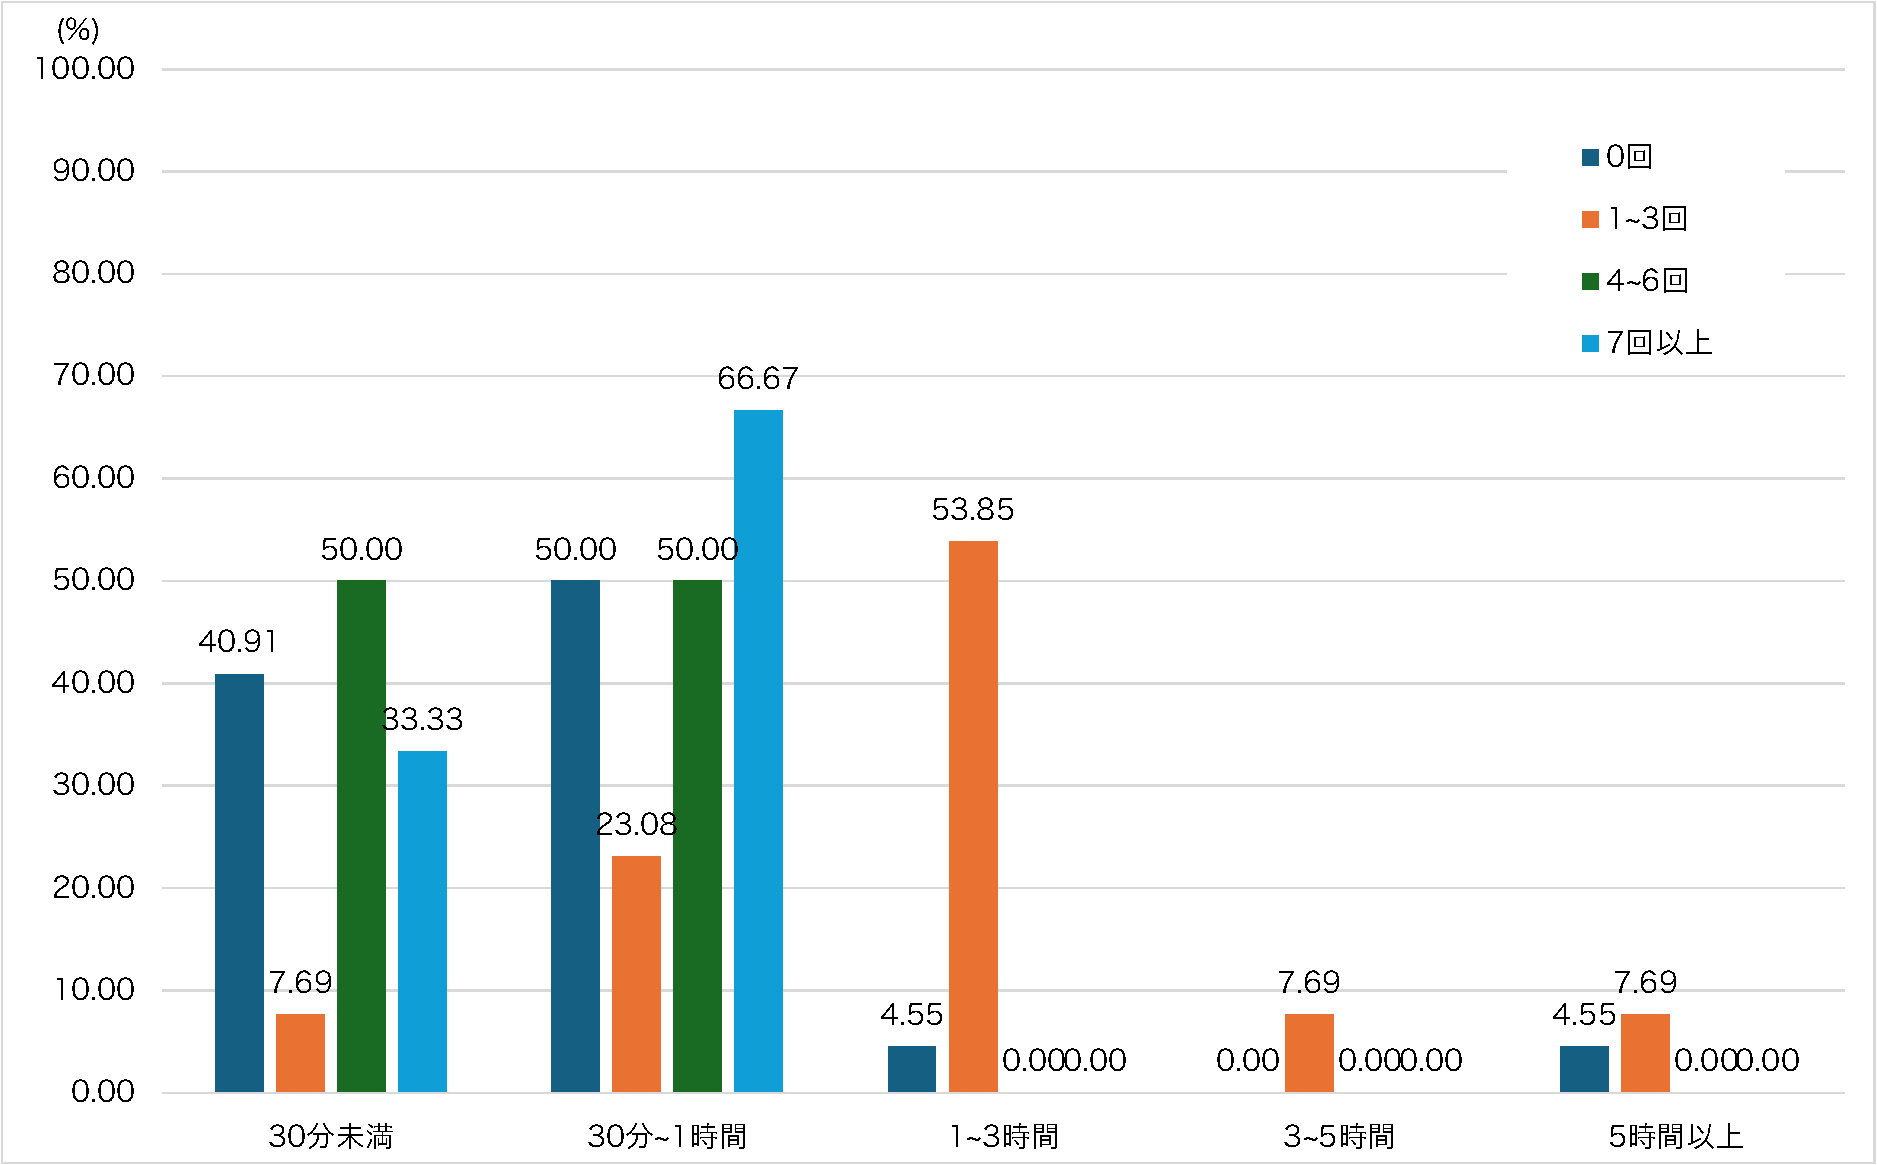
\includegraphics[width=15cm]{視聴回数別学習時間.pdf}
  \caption{提供したコンテンツを経由した学習時間(問1,問3より)}
  \label{fig:jikan2}
\end{figure}

\clearpage

% 8章 3 2
\subsubsection{学習への関心に関する考察}

「問4.視聴しなかったもしくは,視聴回数が少ない理由を教えてください」の質問に表\ref{tb:anke2_7}の選択肢を設け,学生の学習時間に対する関心について視聴回数が0回と1\textasciitilde3回の学生に分けて調査した.
その結果を図\ref{fig:rikai},\ref{fig:yuueki},\ref{fig:mendo}に示す.

視聴回数が0回の学生は視聴しなかった理由として理解できている割合が少なく,面倒だと感じる割合が多い.
加えて学習時間が1時間未満の割合が多い.
これらのことから,学習をする際に心理的な要因が大きく働いており,学習への関心が低いことがわかる.
一方視聴回数が1\textasciitilde3回の学生は理解できている割合と面倒だと感じる割合が多い.
しかし,学習時間が1時間未満の割合は少ないことから心理的な要因は大きいけれど学習への関心はあることがわかる.
視聴回数が1\textasciitilde3回の学生は問2,3のグラフからも学習への関心が高く,提供したコンテンツは学習する際の確認として利用していたと考えられる.
また,図\ref{fig:yuueki}から,コンテンツが有益であると回答したにも関わらず,授業資料へ促せなかった理由として,コンテンツ内容の他に学生の心理的要因が大きく関わっていると考えられる.


%表14
\begin{table}[htbp]
  \caption{問4.視聴しなかった理由の選択肢}
  \begin{center}
\begin{tabular}{ll}\hline
選択肢 & 項目\\ \hline
               1 & 理解できているから\\
               2 & 面倒だから\\
               3 & 有益な情報ではないから\\
               4 & その他\\
               \hline
                \end{tabular}
                \end{center}
                \label{tb:anke2_7}
                \end{table}

%図24~26
\begin{figure}[!htb]
\centering
    \centering
    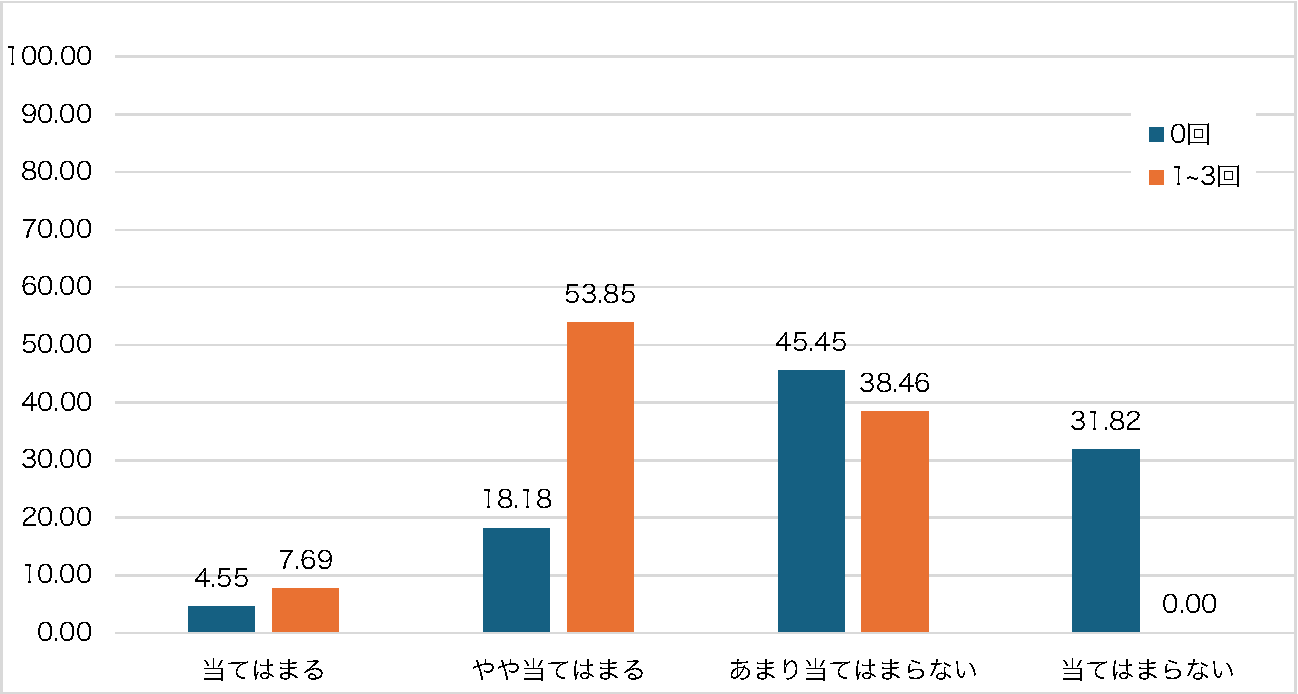
\includegraphics[width=1.0\columnwidth]{理解できているから.pdf}
    \caption{視聴回数が少ない理由:理解できているから(問1,4より)}
    \label{fig:rikai}
\end{figure}

\begin{figure}[!htb]
\centering
    \centering
    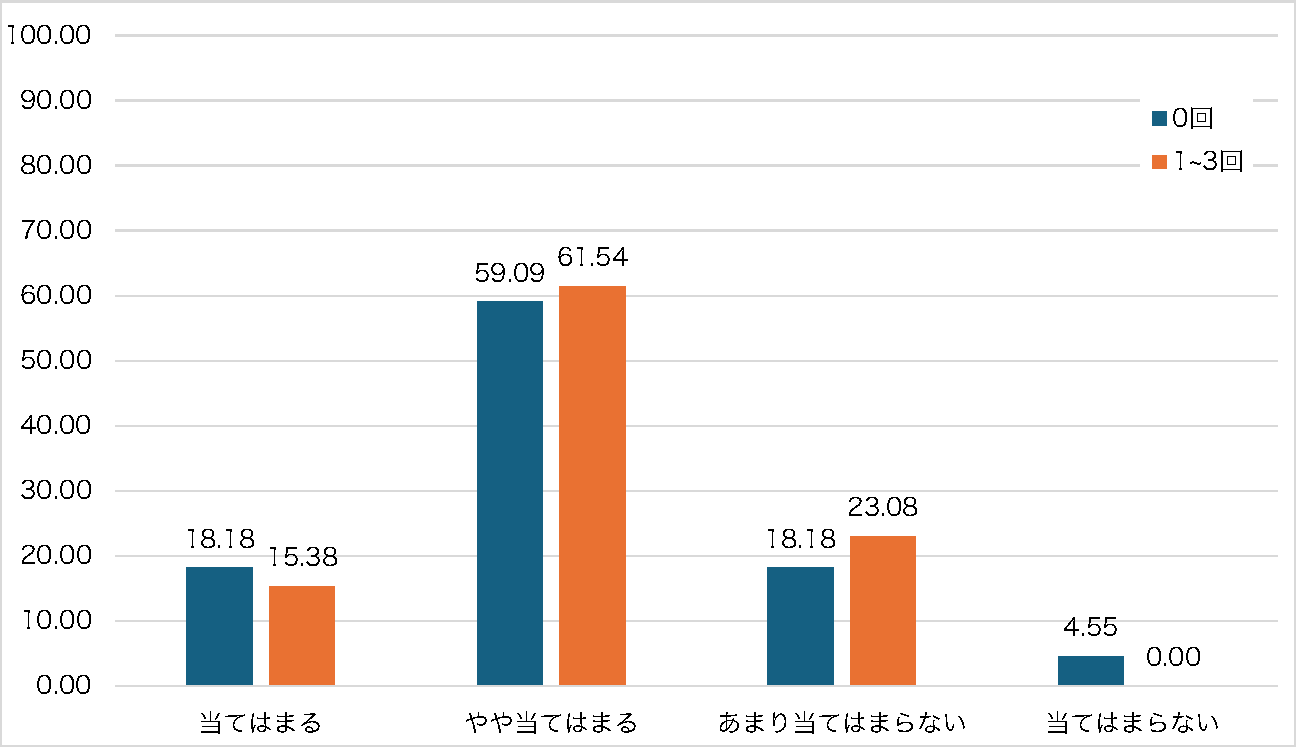
\includegraphics[width=1.0\columnwidth]{面倒だから.pdf}
    \caption{視聴回数が少ない理由:面倒だから(問1,4より)}
    \label{fig:mendo}
\end{figure}

%図を変える!
\begin{figure}[!htb]
\centering
    \centering
    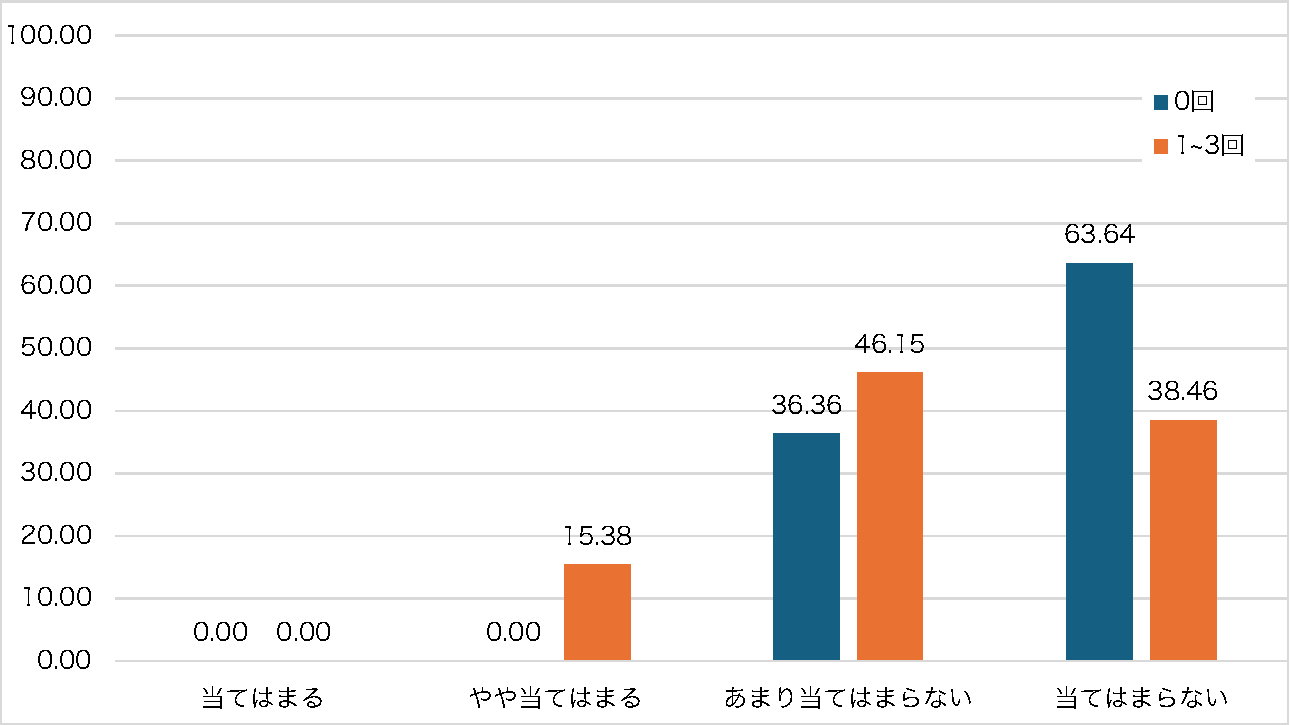
\includegraphics[width=1.0\columnwidth]{有益な情報ではないから.pdf}
    \caption{視聴回数が少ない理由:有益な情報ではないから(問1,4より)}
    \label{fig:yuueki}
\end{figure}

\clearpage

% 8章 3 3
\subsubsection{提供した動画コンテンツの形式に関する考察}

視聴回数が4\textasciitilde6回,7回以上の学生には提供した動画コンテンツについて評価してもらった.
問4\textasciitilde6には表\ref{tb:anke2_5},問7には表\ref{tb:anke2_9}の選択肢を設けた.
表\ref{tb:anke2_6}に質問と評価の平均を示す.
問4\textasciitilde6の質問の回答結果の平均はそれぞれ3.0以上と高く,「問7.提供した動画の時間は適切でしたか」の質問では7人中6人がちょうどいいと回答した.

%表15
\begin{table}[htbp]
  \caption{問4\textasciitilde6の選択肢}
  \begin{center}
\begin{tabular}{ll}\hline
選択肢 & 項目\\ \hline
               1 & 当てはまらない \\ 
               2 & あまり当てはまらない\\
               3 & やや当てはまる\\
               4 & 当てはまる\\
              \hline
               \end{tabular}
               \end{center}
               \label{tb:anke2_5}
               \end{table}

%表16
\begin{table}[htbp]
  \caption{問7の選択肢}
  \begin{center}
\begin{tabular}{ll}\hline
選択肢 & 項目\\ \hline
               1 & 短い \\ 
               2 & ちょうどいい\\
               3 & 長い\\
              \hline
               \end{tabular}
               \end{center}
               \label{tb:anke2_5}
               \end{table}

%表17
\begin{table}[htbp]
  \caption{提供した動画コンテンツの評価}
  \begin{center}
\begin{tabular}{l|llll|l}\hline
               質問 & 1 & 2 & 3 & 4 & 評価平均 \\ \hline
               問4.授業の振り返りとして有効でしたか & 0人 & 0人 & 4人 & 3人 & 3.43\\
               問5.学習コンテンツとして動画の形式は適切だと思いますか & 0人 & 0人 & 2人 & 5人 & 3.71\\
               問6.プレイリストのような工夫は有効だと思いますか & 0人 & 0人 & 0人 & 7人 & 4\\
              \hline
               \end{tabular}
               \end{center}
               \label{tb:anke2_6}
               \end{table}

\clearpage

% 8章 3 4
\subsubsection{学習ツールに関する考察}
また,各授業ごとに利用した学習ツールについての質問では表\ref{tb:anke2_4}の選択肢を設け,調査を行った.
図\ref{fig:tu-ru}に各授業ごとの結果を示す.
どの授業でも選択肢1のmanabaで配布されていた授業資料(文字ベースのPDF)という回答が半分を超えていることから,学生は学習する際に授業資料を利用していることがわかる.
しかし,学習時間に関するアンケートの結果から学生の学習時間が少ないことを再確認できる.

%このことから学生は学習する際に授業資料を使用していることが分かった.
%しかし,学習時間は少ないため,「授業資料の導入となるコンテンツが必要である」という仮説は立証できた.

%表15
\begin{table}[htbp]
  \caption{各授業ごとに利用した学習ツールの質問に対する選択肢}
  \begin{center}
\begin{tabular}{ll}\hline
選択肢 & 学習ツール\\ \hline
               1 & manabaで配布されていた授業資料(文字ベースのPDF)\\
               2 & manabaで配布されていた授業スライド\\
               3 & 提供した学習コンテンツ\\
               4 & その他学部で提供されているコンテンツ(書籍や動画など)\\
               5 & 自主学習していない\\
              \hline
               \end{tabular}
               \end{center}
               \label{tb:anke2_4}
               \end{table}

%図27
\begin{figure}[!htb]
  \centering
  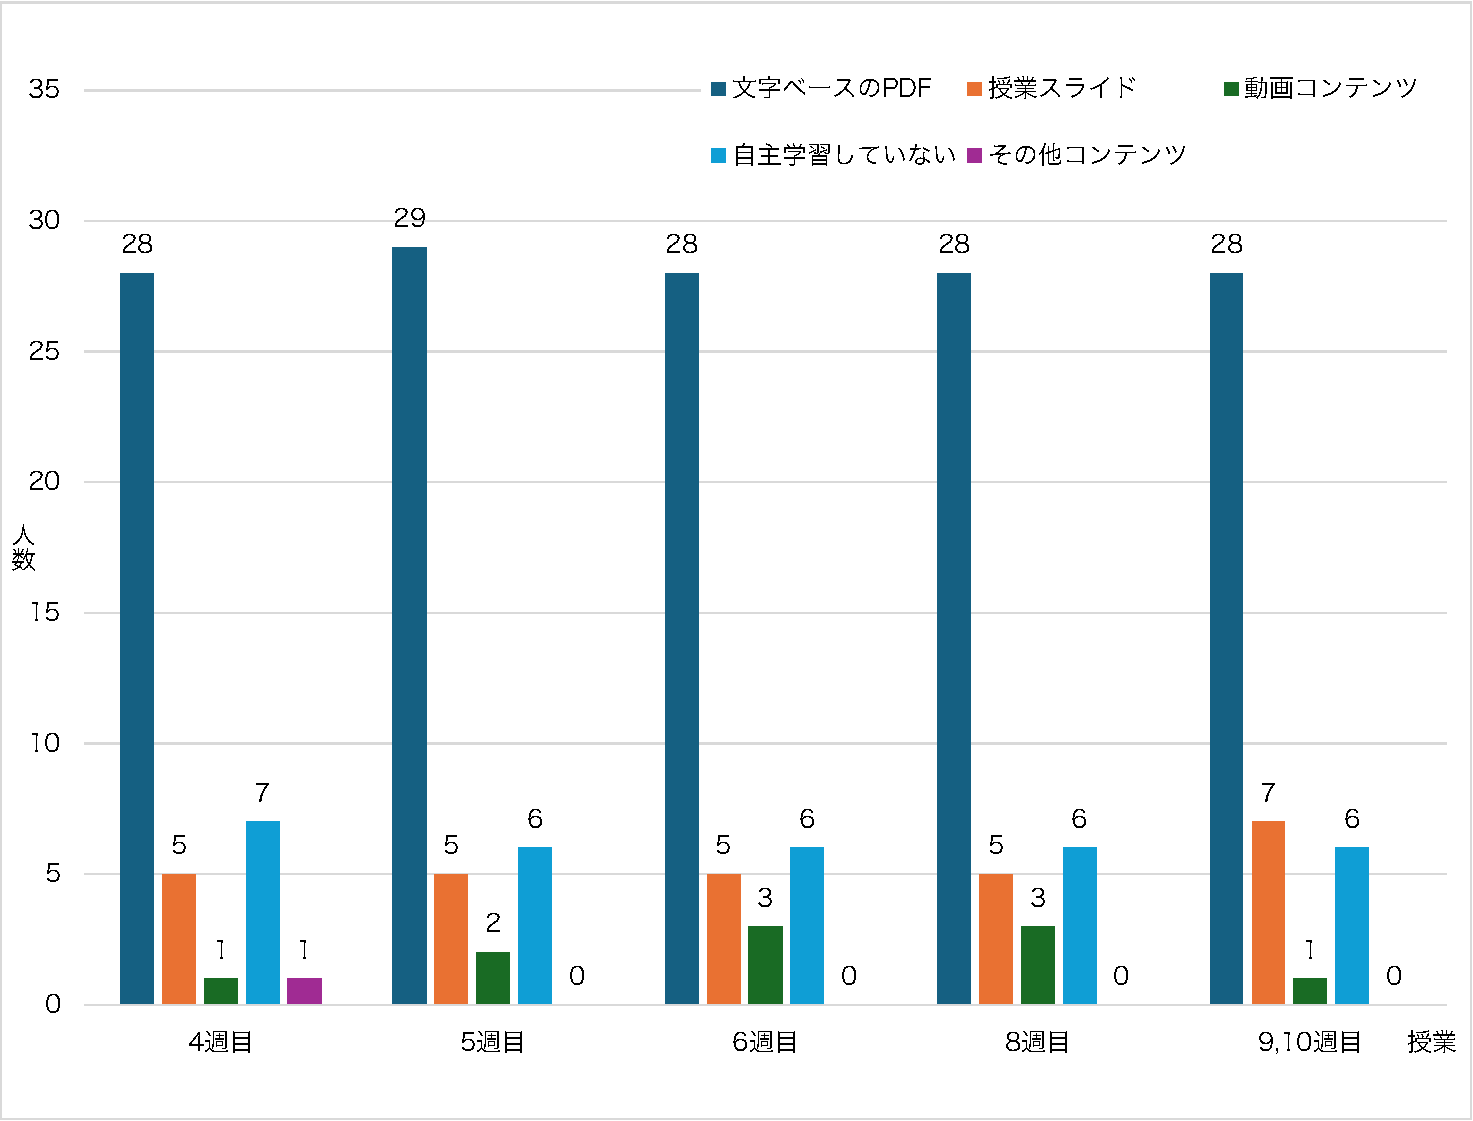
\includegraphics[width=15cm]{各授業ごとの学習ツール.pdf}
  \caption{各授業ごとの学習ツール}
  \label{fig:tu-ru}
\end{figure}


今回,コンテンツ自体の評価はよかったが,学習時間の減少に対する効果は得られなかった.
提供した動画コンテンツは学習意欲が高い学生が確認として利用していたため,本研究の目的であった「学習習慣がない学生には授業内容に沿った導入コンテンツが必要である」という仮説は成立しなかった.
その要因として自主学習をしていない学生には別の心理的な要因があると考えられる.

\clearpage

%9章
\section{結言}
日本では長年,グローバル化に対応した人材の育成を大学に求めている\cite{monka1}.
しかし,学生の学力は低下しつつあるため,求められている能力の育成は行われていないと考えられる.
学生の学力が低下した要因として,専門知識の学習により知識の積み重ねが重要になっていることが挙げられる.
そのため,授業内で配布される資料は以前学習したことの積み重ねができていないと難しいと感じてしまい,学習への抵抗が生まれてしまうという問題点がある.

スマートフォン(スマホ)が普及してから学生は娯楽だけでなく学習する際もスマホを利用するようになっている.
しかし,スマホ上にある学習するコンテンツは知識が点在しているため,自主学習をしてこなかった人にとって知識を積み重ねることは難しく,最終的に授業内容を理解しきれないという問題がある.

今回,「授業資料を用いた自主学習には導入となるコンテンツが必要である」という仮説のもと学生の身近にあるスマホで扱えるコンテンツを提供し,自主学習への繋がりについて検証した.
事前調査として学生の自主学習状況や学習におけるスマホの利用についてアンケートを行い,提供後の調査として提供したコンテンツの評価を行った.
事前調査では十分な時間の学習をしている学生が少ないことや学習する際にはネット上のコンテンツを頼っているということが分かった.
評価のアンケートではコンテンツの視聴が面倒だと感じる学生が多く,学習時間の減少に対する効果は得られなかった.
また,学生の学習意欲によってはコンテンツを自身の学習の補助教材として使用しており,授業資料への導入というコンテンツの目的は達成されなかった.
そのため,「学習習慣がない学生には授業内容に沿った導入コンテンツが必要である」という仮説は成立しなかった.
今後は学生の学習への関心について分析していき,自主学習に繋がるような要因を検討していく予定である.

\clearpage

\begin{thebibliography}{99}
\bibitem{monka1}文部科学省: "大学で育成する人材像と大学政策",\url{https://www.mext.go.jp/b_menu/shingi/chukyo/chukyo0/gijiroku/__icsFiles/afieldfile/2012/03/22/1318900_7.pdf}
\bibitem{monka2}文部科学省: "大学教育改革の状況と厳しい評価",\url{https://www.mext.go.jp/a_menu/koutou/daigakukyou/__icsFiles/afieldfile/2012/04/19/1319974_01.pdf}
\bibitem{monka}文部科学省: "全国学生調査",\url{https://www.mext.go.jp/content/20230712-koutou02-000001987_1.pdf}
\bibitem{chiba}千葉工業大学: "学生生活アンケート2023",\url{https://www.it-chiba.ac.jp/media/2023questionnaire.pdf}
\bibitem{somu1}総務省: "情報通信白書 令和元年版",\url{https://www.soumu.go.jp/johotsusintokei/whitepaper/ja/r01/html/nd111110.html}
\bibitem{somu6}総務省: "情報通信白書 令和6年版",\url{https://www.soumu.go.jp/johotsusintokei/whitepaper/ja/r06/html/nd21b120.html}
\bibitem{somu2}総務省: "令和5年通信利用動向調査の結果",\url{https://www.soumu.go.jp/johotsusintokei/statistics/data/240607_1.pdf}
\bibitem{soumu28}総務省: "情報通信白書 平成28年版",\url{https://www.soumu.go.jp/johotsusintokei/whitepaper/ja/h28/html/nc142120.html}
\bibitem{nomura}野村総合研究所: "日本のChatGPT利用動向",\url{https://www.nri.com/jp/knowledge/report/20230526_1.html}
\bibitem{naikaku}内閣府: "Society 5.0の実現に向けた教育・人材育成に関する政策パッケージ",\url{https://www8.cao.go.jp/cstp/tyousakai/kyouikujinzai/saishu_print.pdf}
\end{thebibliography}

\end{document}
